\documentclass{beamer}
\usetheme{Darmstadt}
\usecolortheme{default}
\usepackage{draftcopy}
\usepackage{graphicx}
\usepackage{amsmath}
\usepackage{enumerate}
\usepackage{verbatim}
\beamertemplatenavigationsymbolsempty


\title{ECO364 (International Trade) Summer 2016}
\date{June 14, 2016}
\author[Scott Orr]{Scott Orr}
\institute{University of Toronto}

\AtBeginSection[]
{
	\begin{frame}
		\frametitle{Outline}
		\tableofcontents[currentsection]
	\end{frame}
}

\begin{document}
	
	\begin{frame}
		\titlepage
	\end{frame}
	
	\section{Outline}
	
\begin{frame}
	\frametitle{Outline for Today}
	
		\begin{itemize}
			\item Allow for increasing returns in heterogeneous firm models.
			\begin{itemize}
				\item Motivation: Why are exporters more productive?
				\item Heterogeneous Firms with Fixed Costs
				\item Heterogeneous Firms with Exporting Costs
			\end{itemize}
			\item Some empirics.
				\begin{itemize}
					\item Impact of trade liberalization on productivity
				\end{itemize}
			\item External economies of scale.
				\begin{itemize}
					\item Introduction
					\item Model
					\item ``Infant Industry" argument.
				\end{itemize}
		\end{itemize}

\end{frame}

\section{Increasing Returns and Firm Heterogeneity}
\subsection{Motivation: Why are exporters more productive?}

\begin{frame}
	\frametitle{Motivation: Exporters and Productivity}
	
\begin{itemize}
	\item Exporters tend to be ``better" in a number of dimensions, compared to non-exporters. (Bernard and Jensen 1999)
		\begin{itemize}
			\item Relative to plants that only produce for the domestic market, exporters are:
				\begin{itemize}
					\item More capital intensive.
					\item More technology intensive.
					\item Pay higher wages.
					\item Are more productive.
				\end{itemize}
		\end{itemize}
	\item Why is this?

\end{itemize}
\end{frame}

\begin{frame}
	\frametitle{Labour Productivity Of Canadian Manufacturers}

			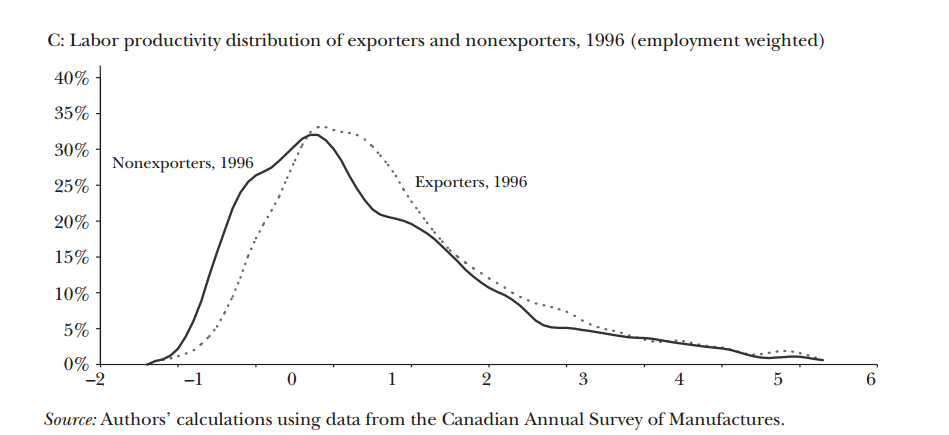
\includegraphics[scale=0.48]{SL4_productivity.png}
			
			\begin{center}
				\scriptsize
				Source: Melitz and Trefler (2012)
			\end{center}

			

\end{frame}

\begin{frame}
	\frametitle{Exporting, Productivity, and Selection}
	
\begin{itemize}
	\item Popular explanation: Highly productive exporters may be due to \emph{selection}
		\begin{itemize}
			\item Since exporting is costly, it may be that only the most productive firms can afford to enter export markets
		\end{itemize}
	\item Note: causality may run in the other direction!
		\begin{itemize}
			\item Exporters may ``learn" to be more productive through exporting.
		\end{itemize}
\end{itemize}

\end{frame}

\begin{frame}
	\frametitle{Exporting, Productivity, and Selection: Theory}
	\begin{itemize}
	\item Whether the exporter ``productivity premium" is due to selection or learning is an empirical question.
	\item We are going to first focus on the theory underlying positive selection of exporters
	\begin{itemize}
		\item How does this export market ``selection effect" interact with the market entry selection effects we discussed last class?
		\item To do this, we need to add fixed costs to the heterogeneous firm model.
	\end{itemize}
\end{itemize}
	
\end{frame}
\subsection{Heterogeneous Firms with Fixed Costs}

\begin{frame}
	\frametitle{Monopolistic competition with heterogeneous firms}

Quick recap of heterogeneous firm model:
	\begin{itemize}
		\item Each firm $j$ faces the same symmetric demand function
		\begin{equation}
		q_j(p_j)=S\left[\frac{1}{n} - b\left(p_j -\bar{p} \right)\right] \nonumber
		\end{equation}
	\item Different firms have different marginal costs $c_j$
		\begin{equation}
		TC_j = c_jq_j \nonumber
		\end{equation}
	\item We showed last class that:
		\begin{itemize}
		\item In equilibrium there is a cutoff marginal cost, $c^*$, such that any firm with $c_j>c^*$ exits the market
		\item Trade integration increases $c^*$, forcing the least productive firms out the market.
		\end{itemize}
	\item Let's now add increasing returns to scale to the model:
			\begin{equation}
			TC_j = c_jq_j + F \nonumber
			\end{equation}
	\item $F$ is not sunk (i.e. rent)!
		
	\end{itemize}

\end{frame}

\begin{frame}
	\frametitle{Heterogeneous Firms and Fixed Costs}

\begin{itemize}
		\item Each firm still prices according to the first-order condition:
		\begin{itemize}
			\item $MR_j=MC_j$
		\end{itemize}
		\item Note that by definition fixed costs do not affect marginal costs.
		\item Pricing rules for firms is exactly the same.
				\begin{equation}
				p_j^*=p^*(c_j)=\frac{1}{2}\left(\frac{1}{bn}+\bar{p} + c_j\right) \nonumber 
				\end{equation}
		\item The addition of fixed costs makes the cutoff marginal cost, $c^*$, lower. 
			\begin{itemize}
				\item No longer equal to the ``choke price"
			\end{itemize}
\end{itemize}
\end{frame}

\begin{frame}
	\frametitle{Cutoff marginal cost with increasing returns to scale}
	
		\frametitle{Pricing, Quantity, and Profits by Costs}
		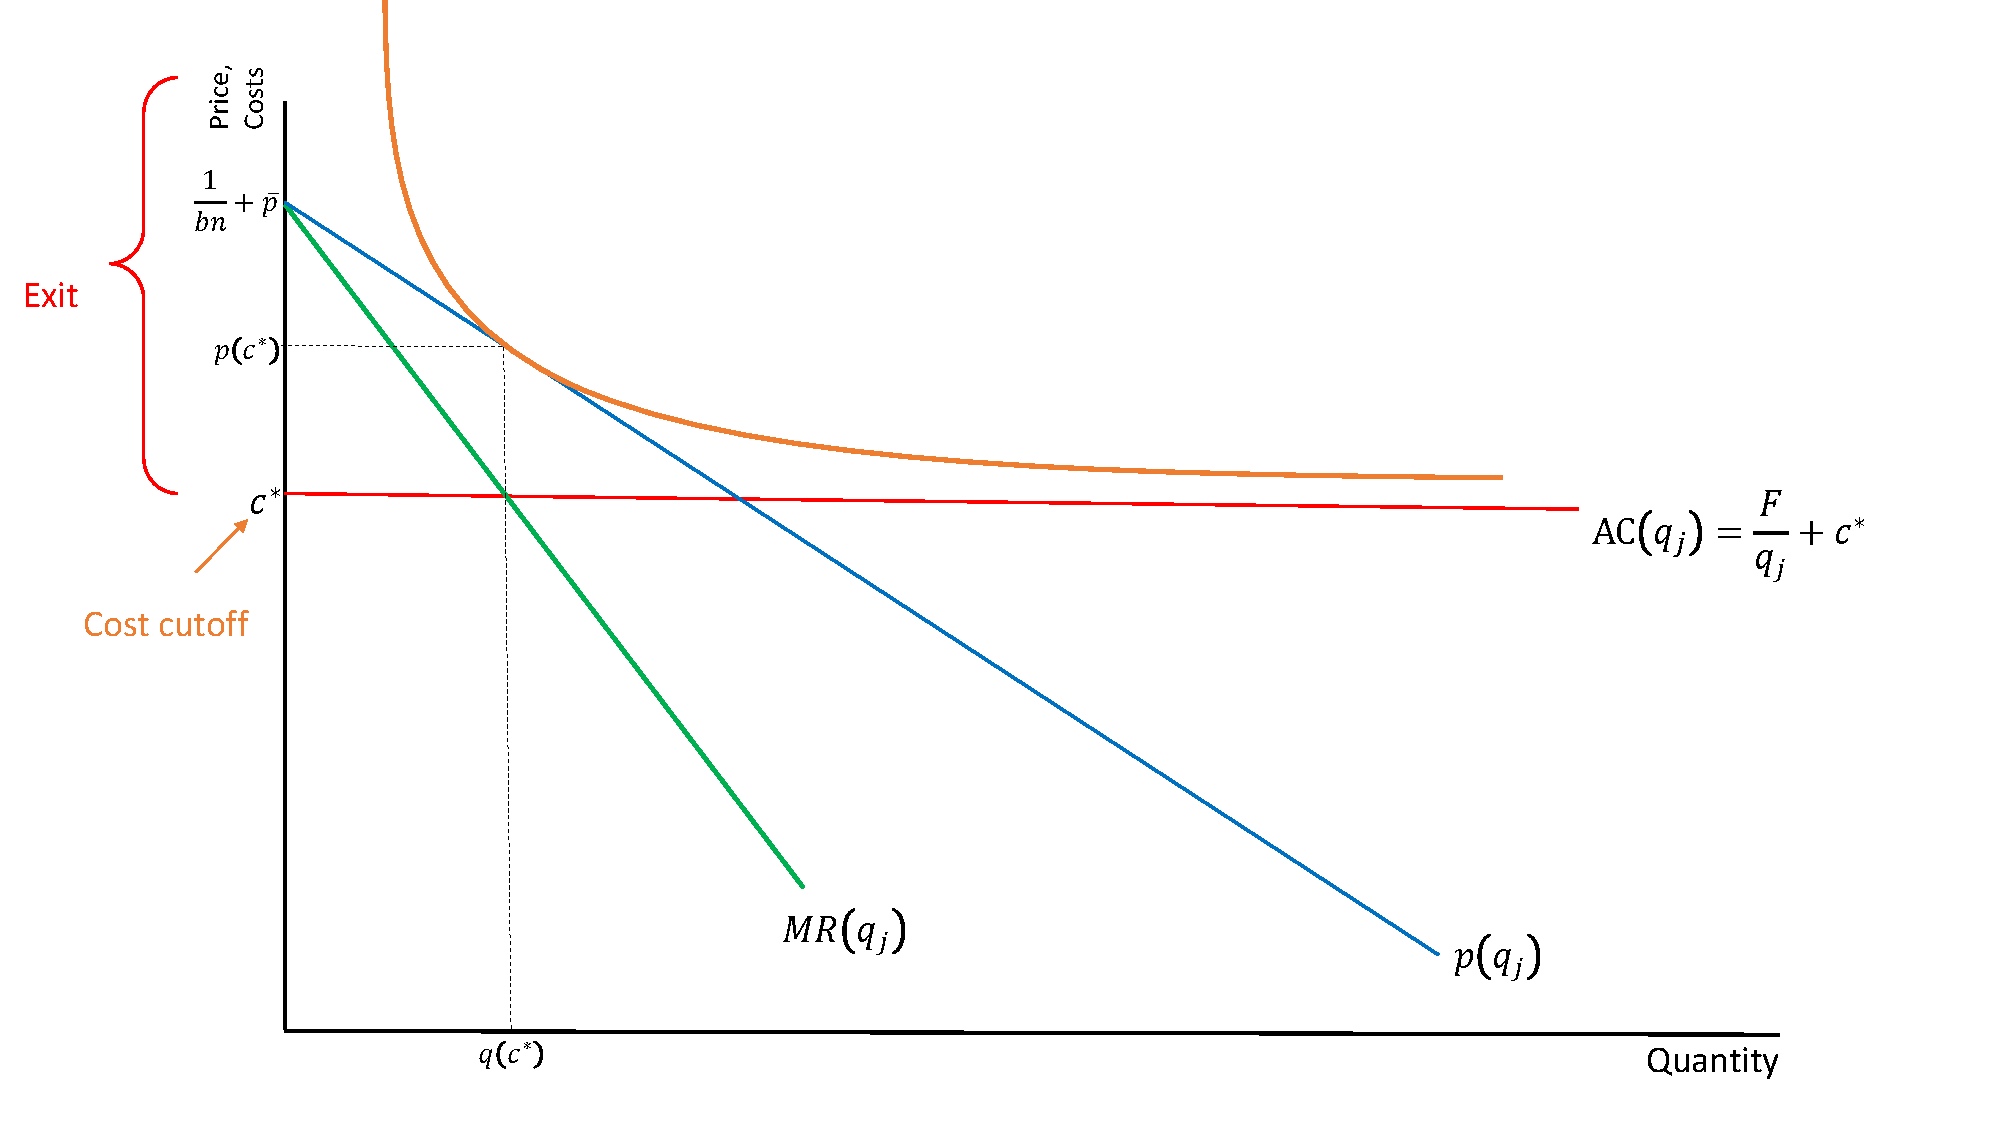
\includegraphics[scale=0.32]{SL4_1.pdf}
		
\end{frame}

\begin{frame}
	\frametitle{Costs, productivity, and profits}
	\begin{itemize}
		\item Since pricing rule has not changed, operating profits simply given by:
					\begin{equation}
					\pi(c_j)=\frac{Sb}{4}\left(\frac{1}{bn}+\bar{p} -c_j \right)^2 -F \nonumber
					\end{equation}
						\begin{itemize}
							\item Lower cost firms still earn higher profits.
							\item $\pi(c^*)=0$ defines the cutoff cost.
									\begin{itemize}
										\item Can use the above expression for $c^*$ algebraically (as a function of $\bar{p},n,S,$ and $F$)
										\item Practice this on your own 
									\end{itemize}
						\end{itemize}
							\item Firms with $c_j > c^* $ exit.
			\end{itemize}

	


\end{frame}

\begin{frame}
	\frametitle{Productivity cutoffs}
	
			\frametitle{Profits for different costs}
			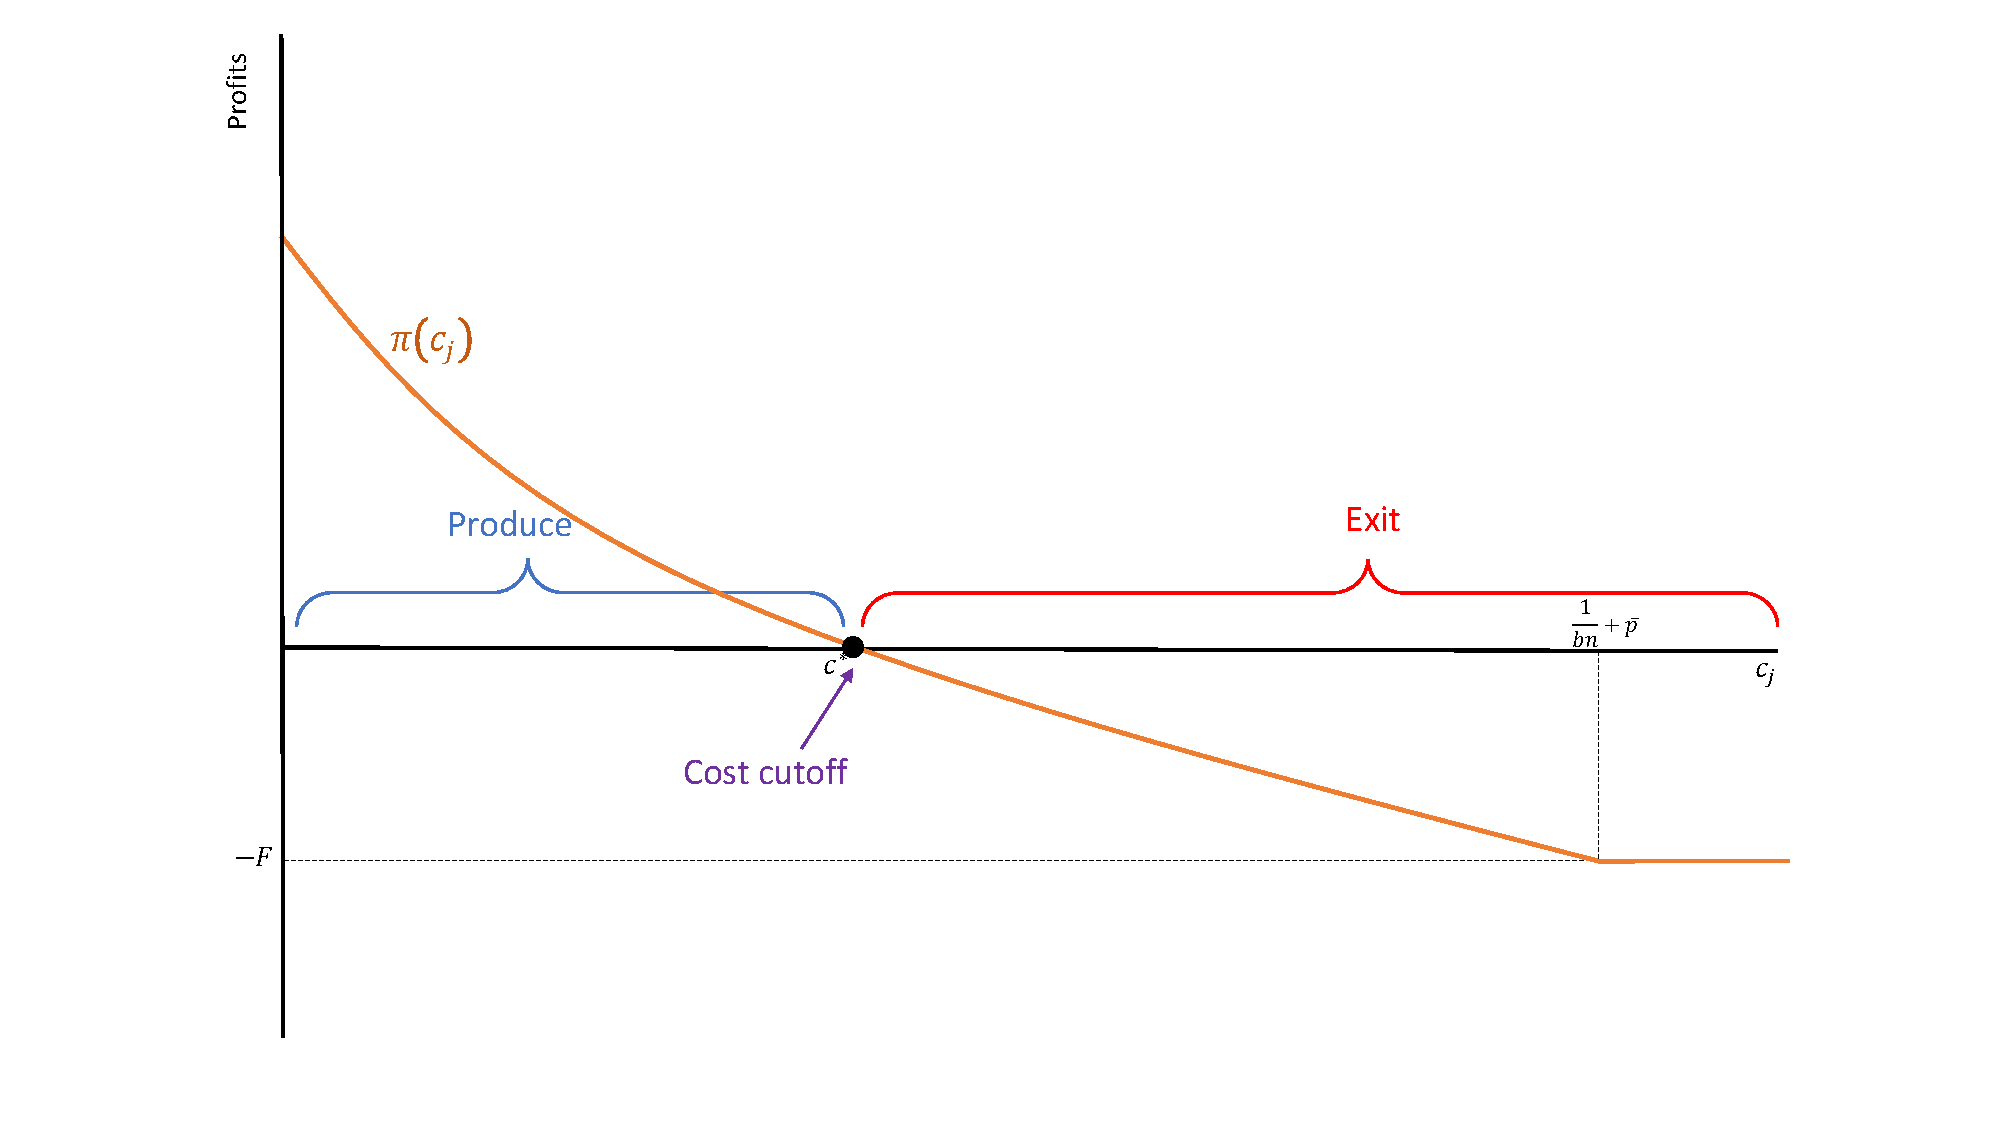
\includegraphics[scale=0.32]{SL4_7.pdf}
	
\end{frame}

\subsection{Heterogeneous Firms with Exporting Costs}
\begin{frame}
	\frametitle{Export market selection}
Now suppose that home ($h$) firms can choose to export to an identical foreign country. 
	\begin{itemize}
		\item Key assumption: Exporting is costly (E.g. Setting up a shipping route)
			\begin{itemize}
				\item Suppose each firm must pay $F_x$ per period to access export market.
					\begin{itemize}
						\item In \emph{addition} to the operating fixed costs $F$.
						\item This guarantees that if a firm exports, they will also serve the domestic market. 
					\end{itemize}
				\item We will just consider fixed costs to exporting.
					\begin{itemize}
						\item We could add variable shipping costs to the model as well, but the qualitative results would not change. 
					\end{itemize}
			\end{itemize}
	\end{itemize}
\end{frame}

\begin{frame}
	\frametitle{Who exports?}
	\begin{itemize}
	\item Key trade-off:
		\begin{itemize}
			\item Larger market: $\pi \uparrow$
			\item But have to pay $F_x$:  $\pi \downarrow$
		\end{itemize}
		\item Only larger, productive firms benefit from increased market size enough to justify paying the export costs:
		\end{itemize}
\end{frame}

\begin{frame}
				\frametitle{Export Versus Dometisc Profits}
				\includegraphics[scale=0.32]{SL4_8.pdf}
\end{frame}

\begin{frame}
	\frametitle{Export Versus Dometisc Profits}
	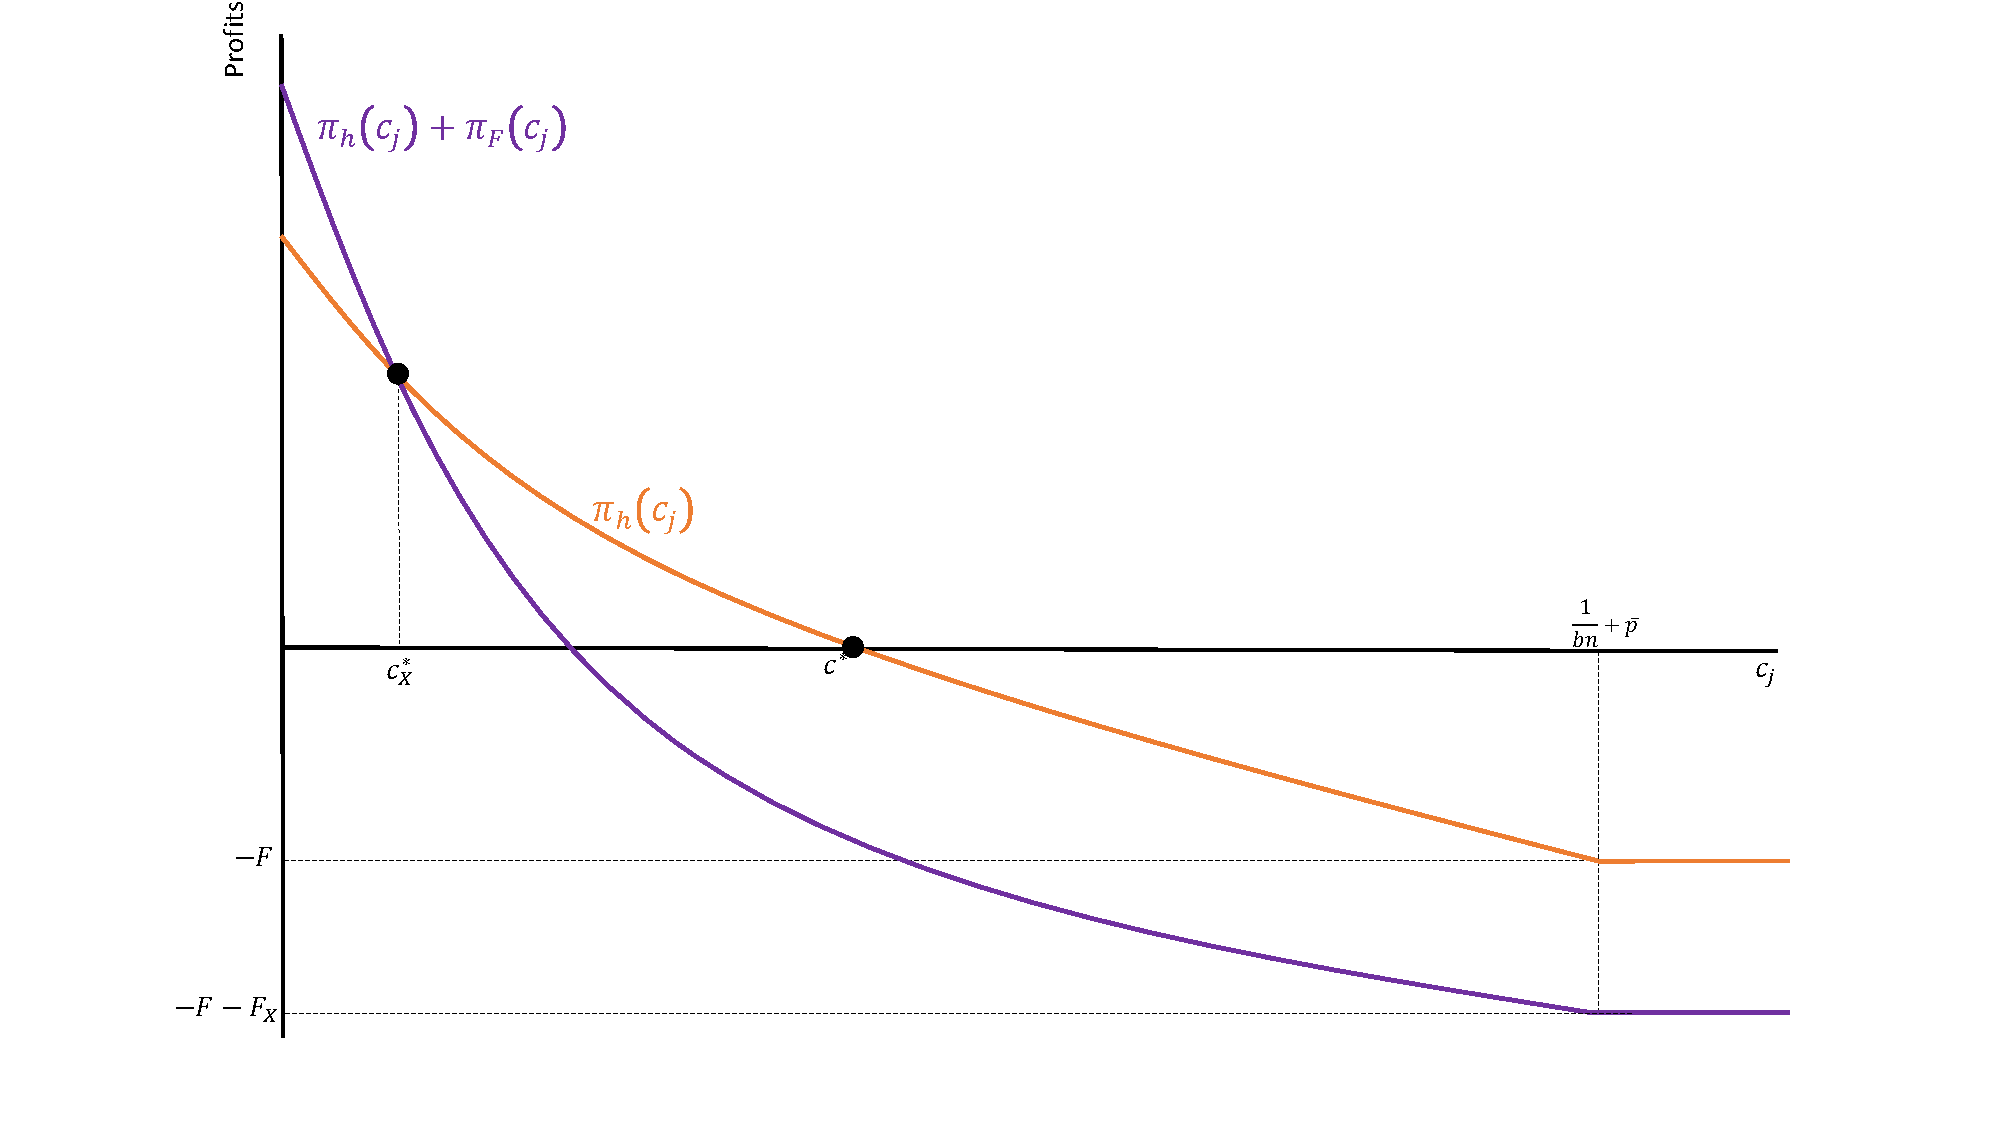
\includegraphics[scale=0.32]{SL4_9.pdf}
	
	
\end{frame}

\begin{frame}
	\frametitle{Export Versus Dometisc Profits}
	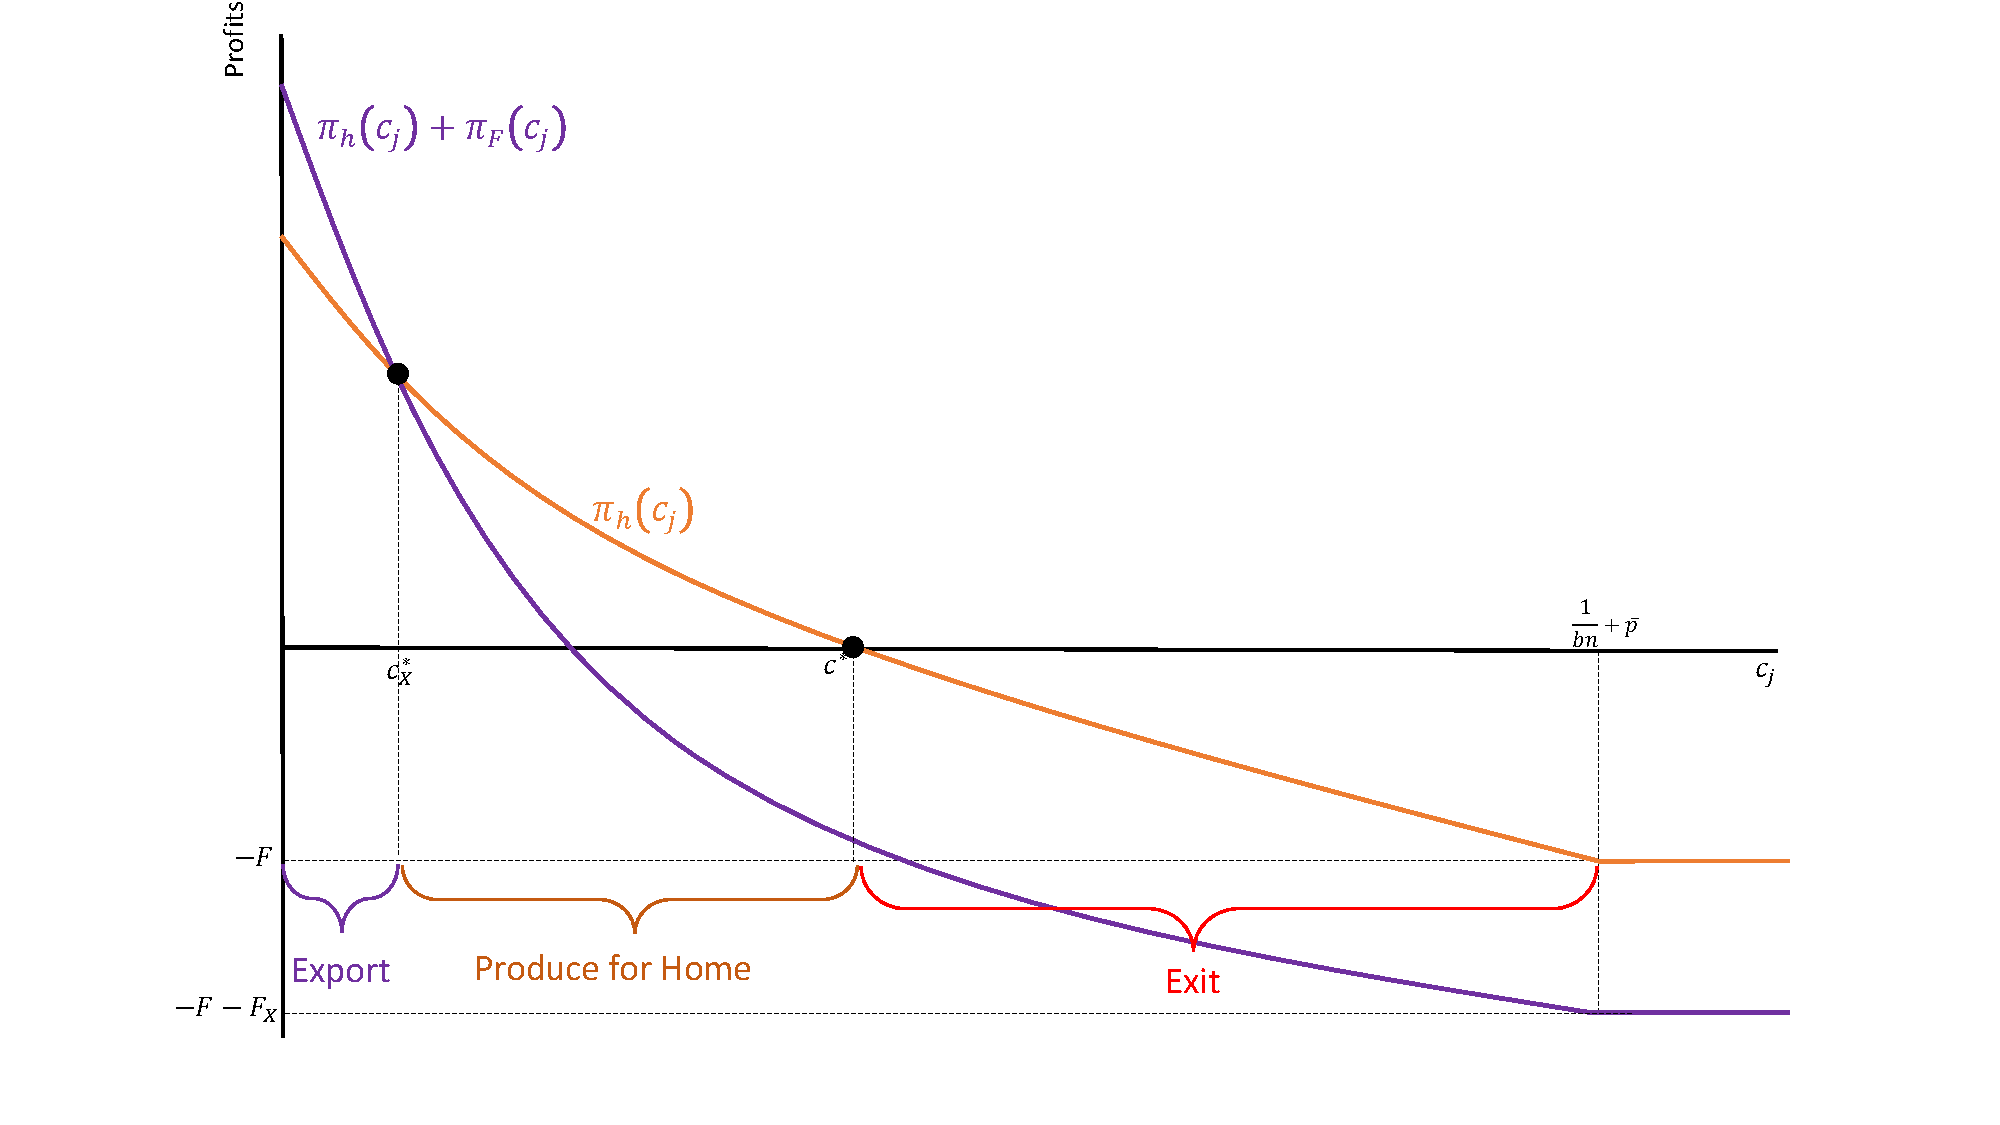
\includegraphics[scale=0.32]{SL4_10.pdf}
	
\end{frame}


\begin{frame}
	\frametitle{Export market selection}
With costly export markets:
	\begin{itemize}
		\item Only highly productive (low cost) firms earn higher profits by exporting	$\rightarrow$ positive selection into export markets.
			\begin{itemize}
				\item Firms with $c\leq c^*_X$
			\end{itemize}
		\item Medium productivity firms only serve the domestic market
					\begin{itemize}
						\item Firms with $c^*_X<c\leq c^*$
					\end{itemize}
		\item Low productivity firms exit.
							\begin{itemize}
								\item Firms with $c^*<c$
							\end{itemize}
	\end{itemize}
\end{frame}
	
\begin{frame}
	\frametitle{Trade liberalization with export costs}
What does trade liberalization do?
	\begin{itemize}
		\item Convenient to think of this as a fall in $F_x$ 
			\begin{itemize}
				\item We shall assume that $F_x$ falls both for the foreign country \emph{and} home country.
			\end{itemize}
	    \item Could also think of this as a fall in variable trade costs, but qualitative results are about the same. 
	\end{itemize}
We shall consider falling trade costs in two steps:
	\begin{enumerate}
		\item Direct effect: Increased access to foreign markets.
		\item Indirect effect: Increased competition.
	\end{enumerate}
\end{frame}


\begin{frame}
	\frametitle{Direct effect of falling export costs}
\begin{itemize}
	\item If it becomes cheaper to enter export markets, we should see more export market entry.
		\begin{itemize}
			\item $c^*_X$ will \emph{fall}.
			\item More firms enter export markets, but these firms are marginally less productive.
		\end{itemize}
\end{itemize}
\end{frame}

\begin{frame}
	\frametitle{Falling Export Costs: Direct Effect}
	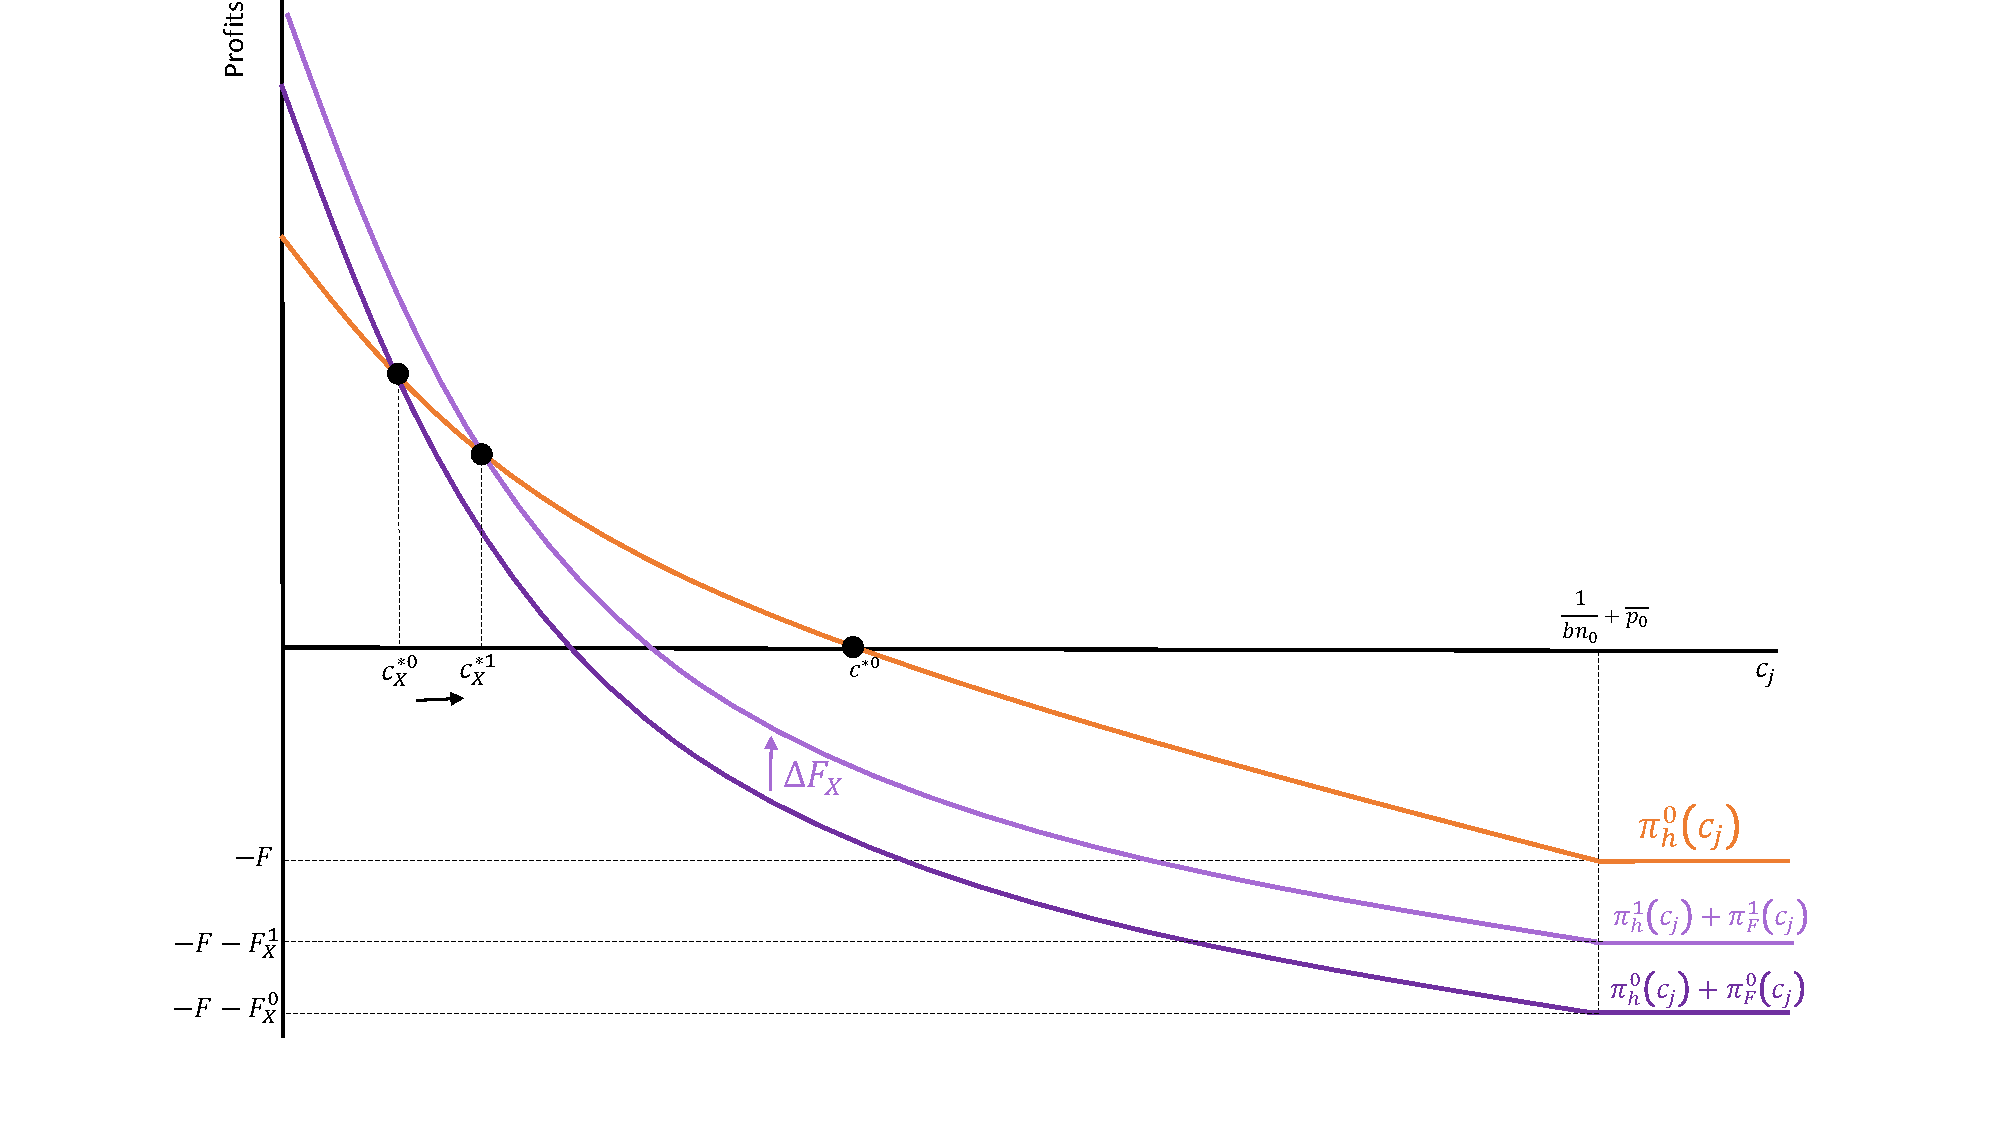
\includegraphics[scale=0.32]{SL4_11.pdf}
	
\end{frame}

\begin{frame}
	\frametitle{Indirect effect of falling export costs: Increased competition}
Recall that we are assuming that $F_x$ is falling in both the home and foreign market.
	\begin{itemize}
		\item Since more home firms enter the export (foreign) market, more foreign firms should enter the home market as well.
		\item Number of firms has to rise $(\uparrow n)$
		\item Extra competition drives down the profits that be earned domestically and by exporting
	\end{itemize}
\end{frame}

\begin{frame}
	\frametitle{Falling Export Costs: Competition Effect}
	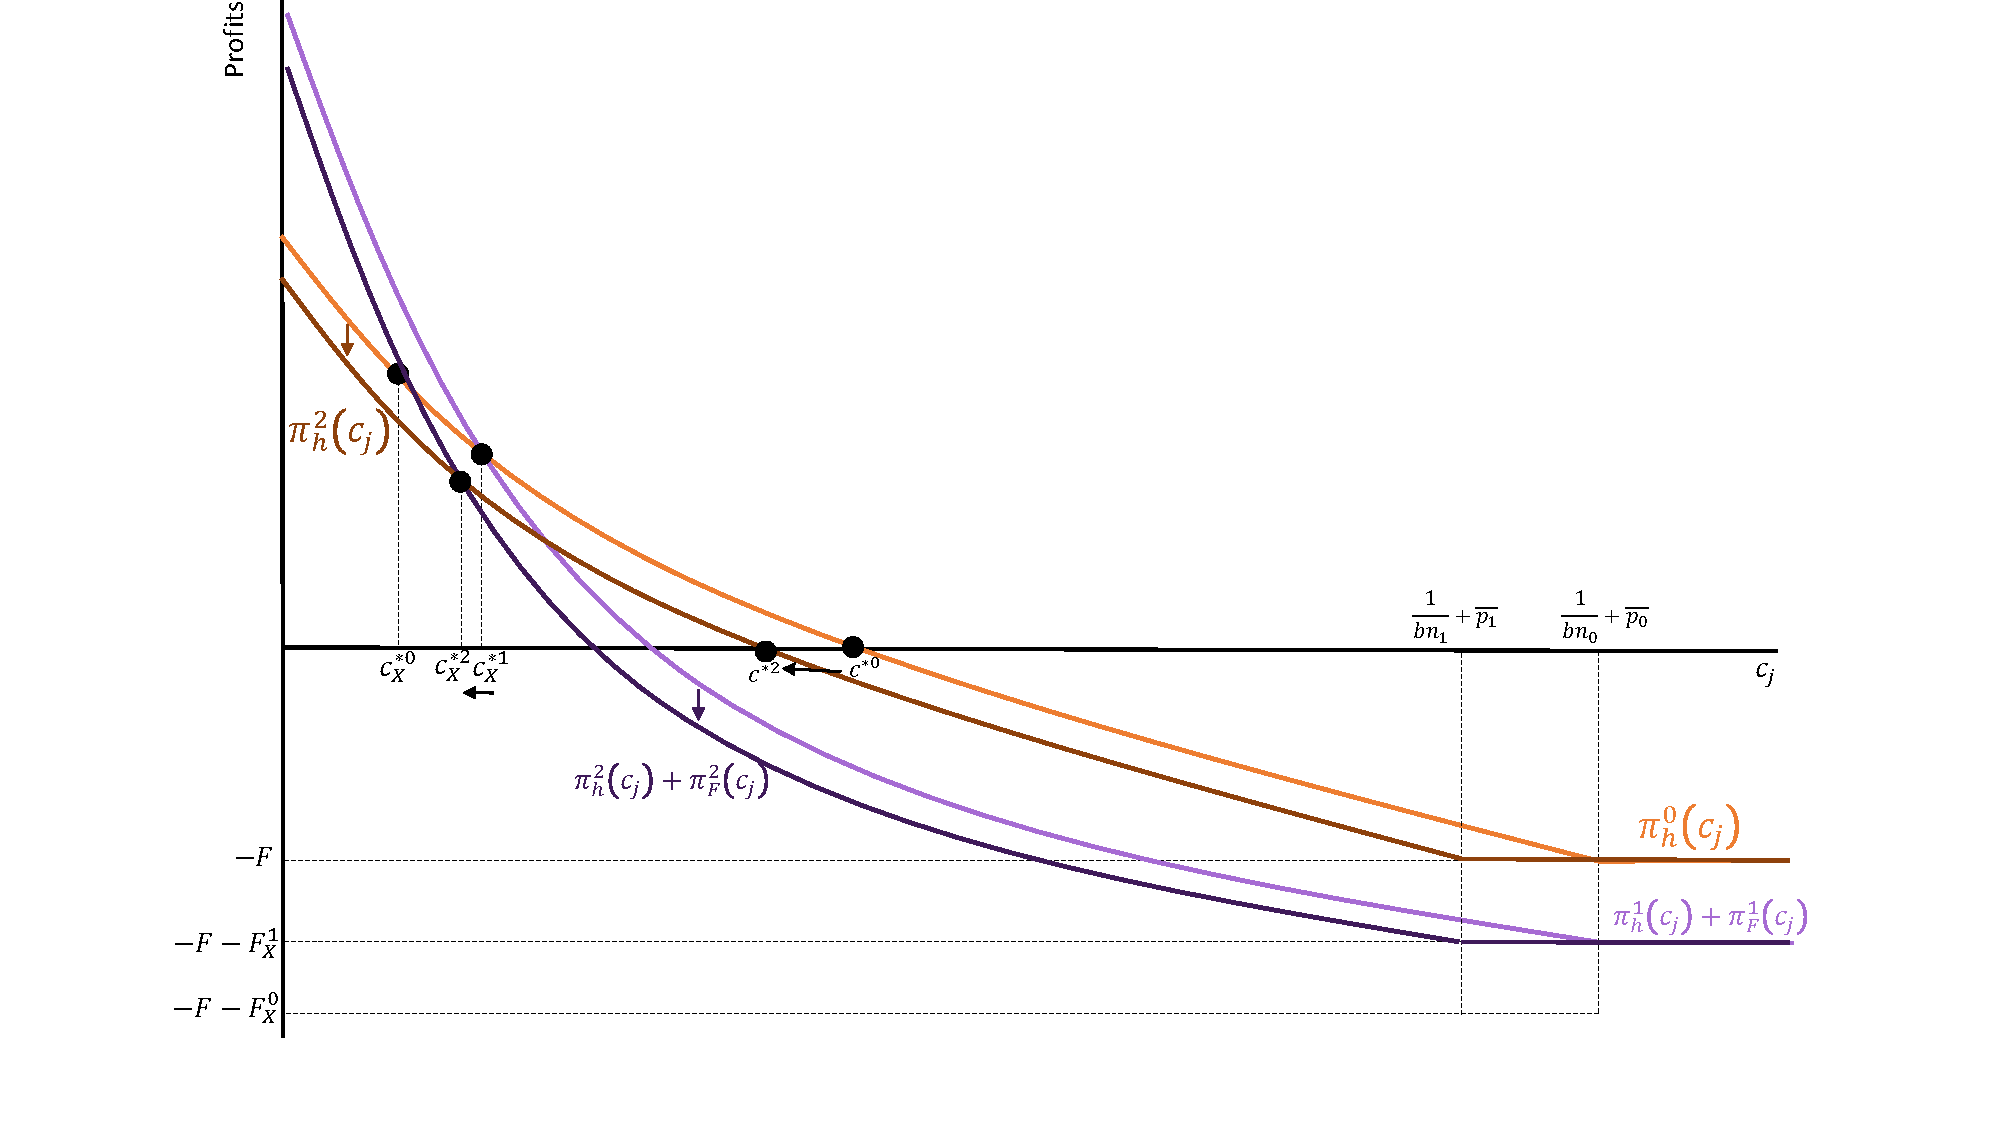
\includegraphics[scale=0.32]{SL4_12.pdf}
	
\end{frame}

\begin{frame}
	\frametitle{Falling Export Costs: Overall Effect}
	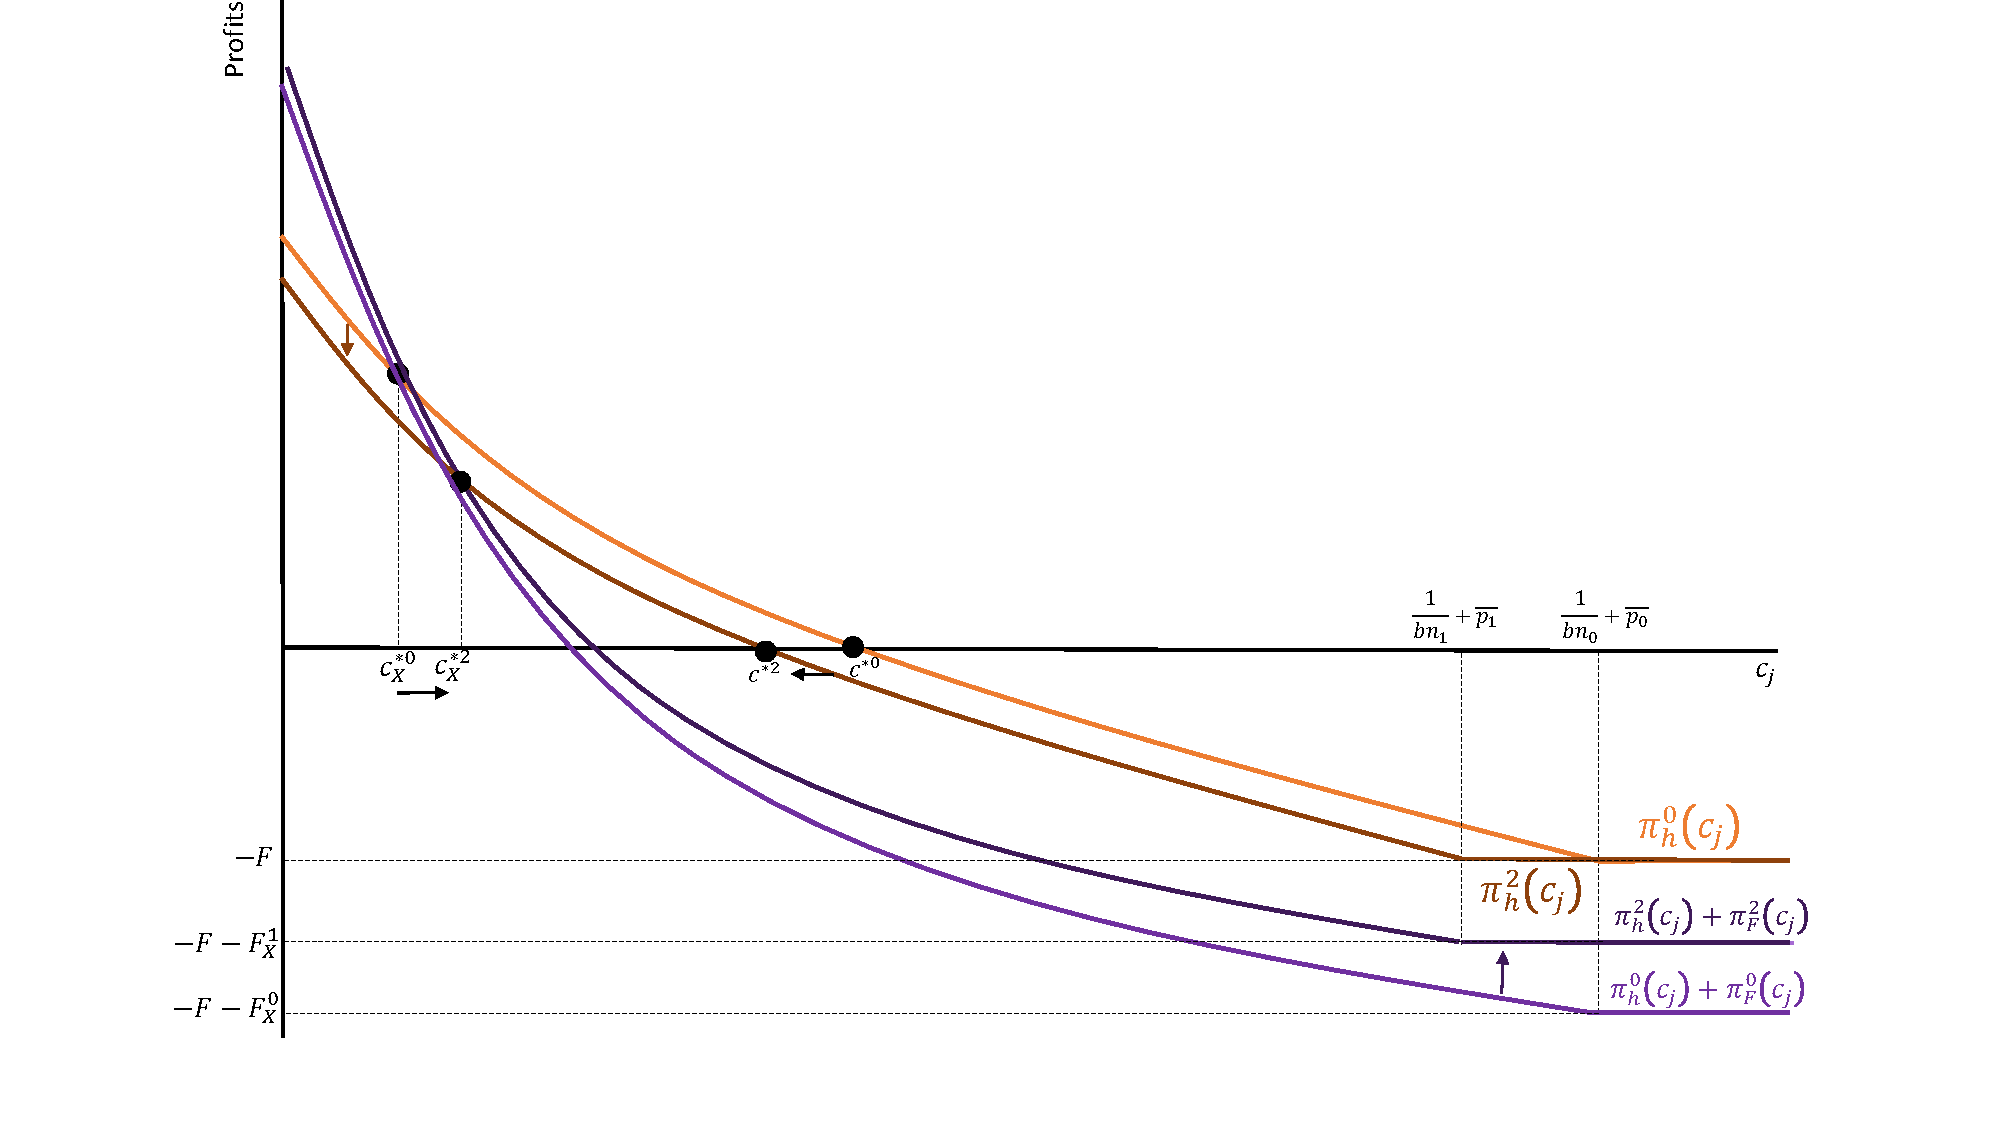
\includegraphics[scale=0.32]{SL4_13.pdf}
	
\end{frame}

\begin{frame}
	\frametitle{Falling Export Costs: Initial Cost Cutoffs}
	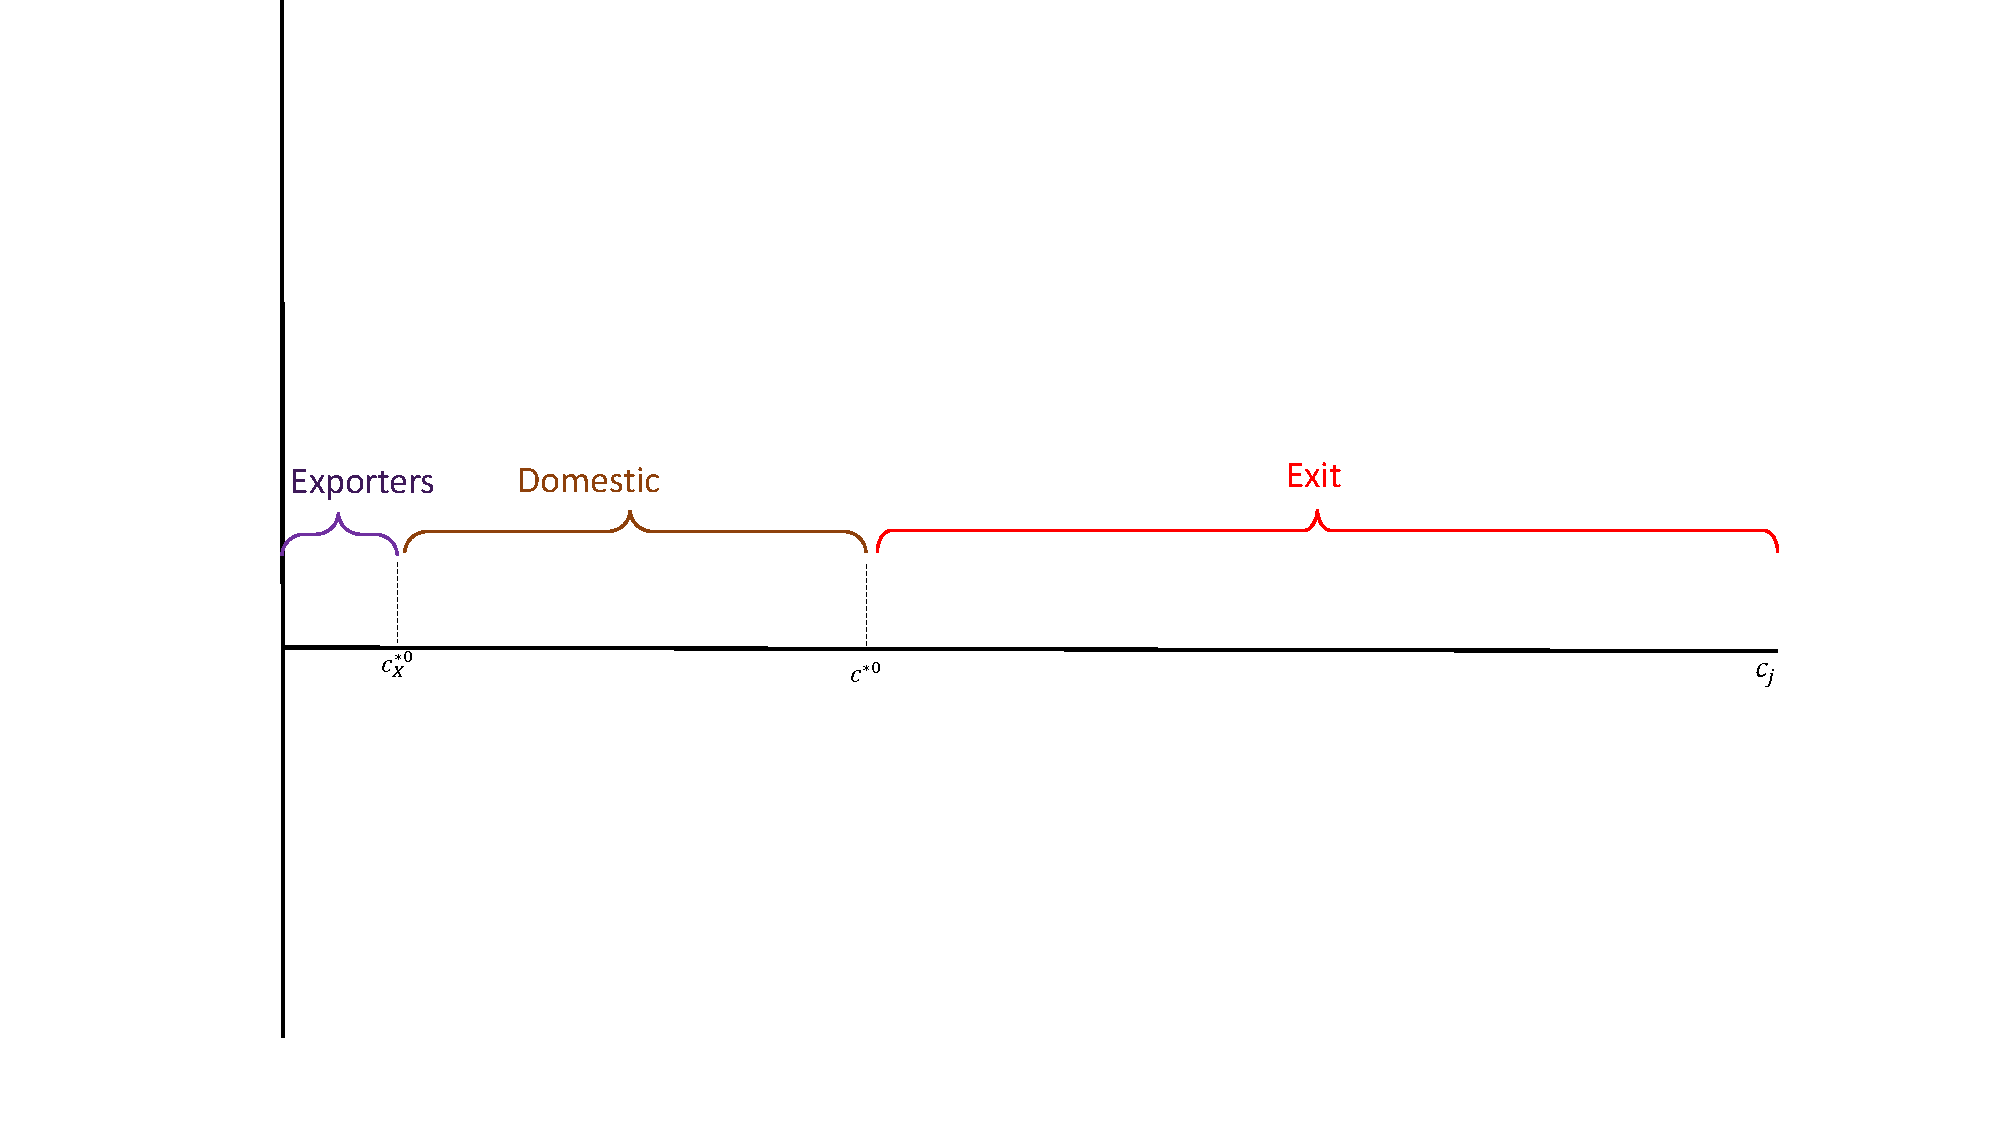
\includegraphics[scale=0.32]{SL4_27.pdf}
	
\end{frame}

\begin{frame}
	\frametitle{Falling Export Costs: Change in Cost Cutoffs}
	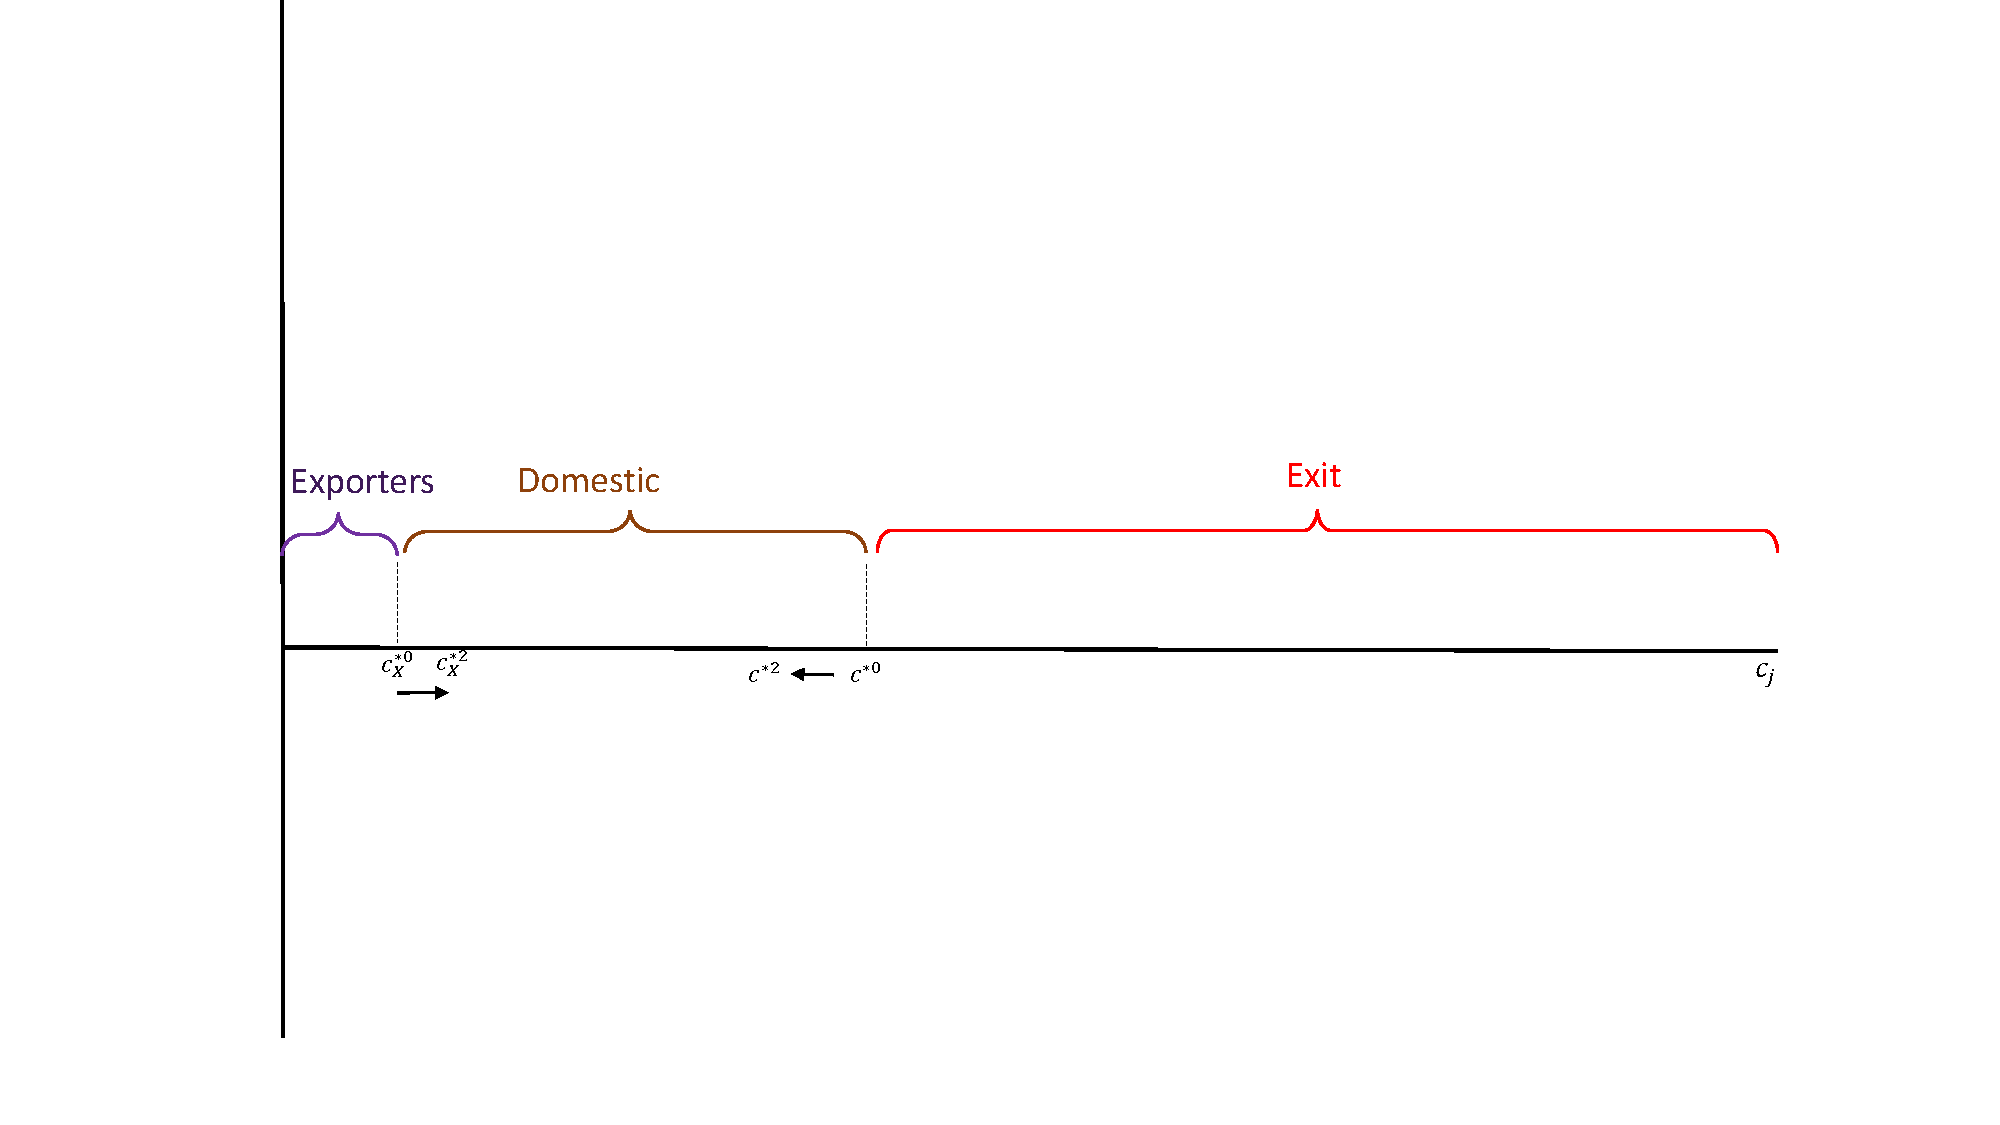
\includegraphics[scale=0.32]{SL4_28.pdf}
	
\end{frame}

\begin{frame}
	\frametitle{Falling Export Costs: Entry and Exit}
	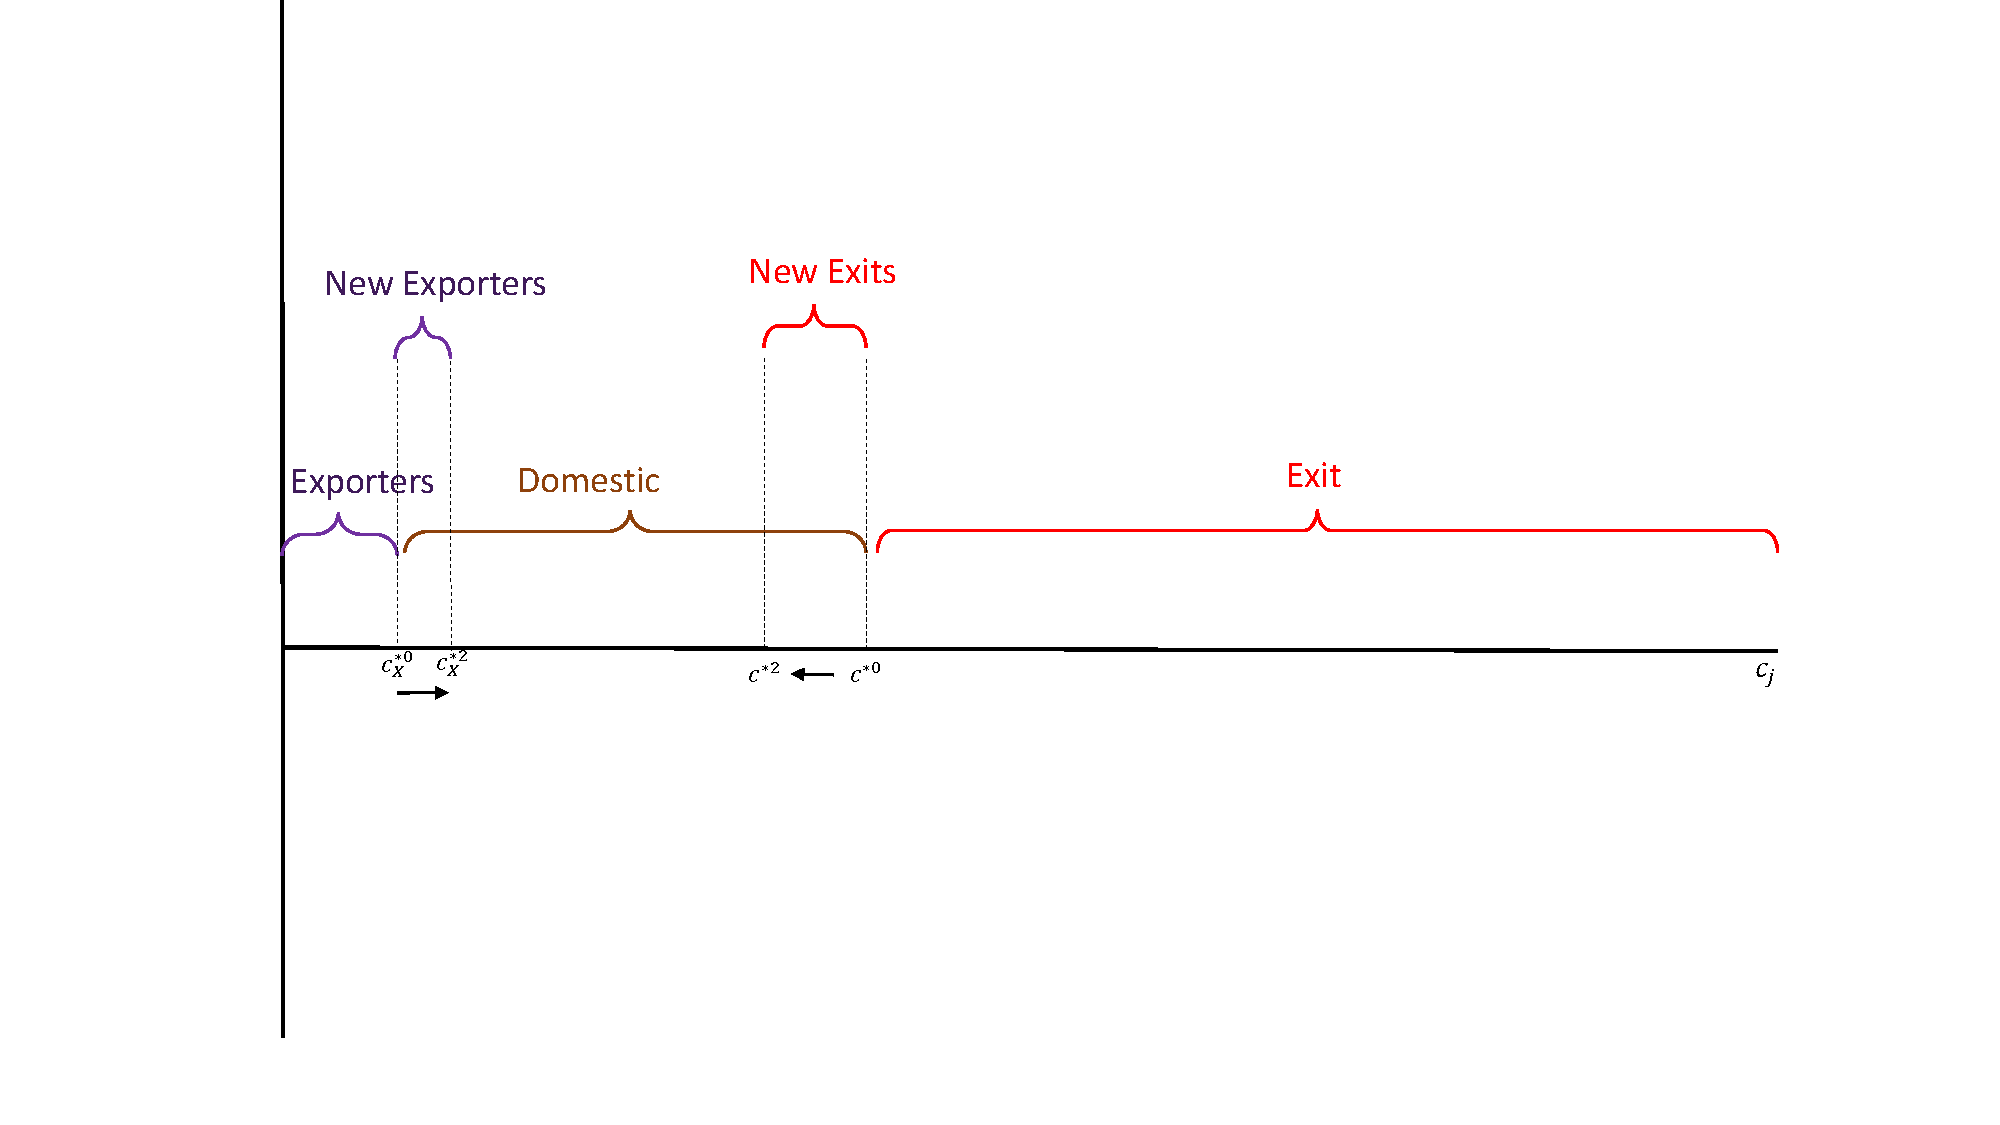
\includegraphics[scale=0.32]{SL4_29.pdf}
	
\end{frame}

\begin{frame}
	\frametitle{Falling Export Costs: Final Cost Cutoffs}
	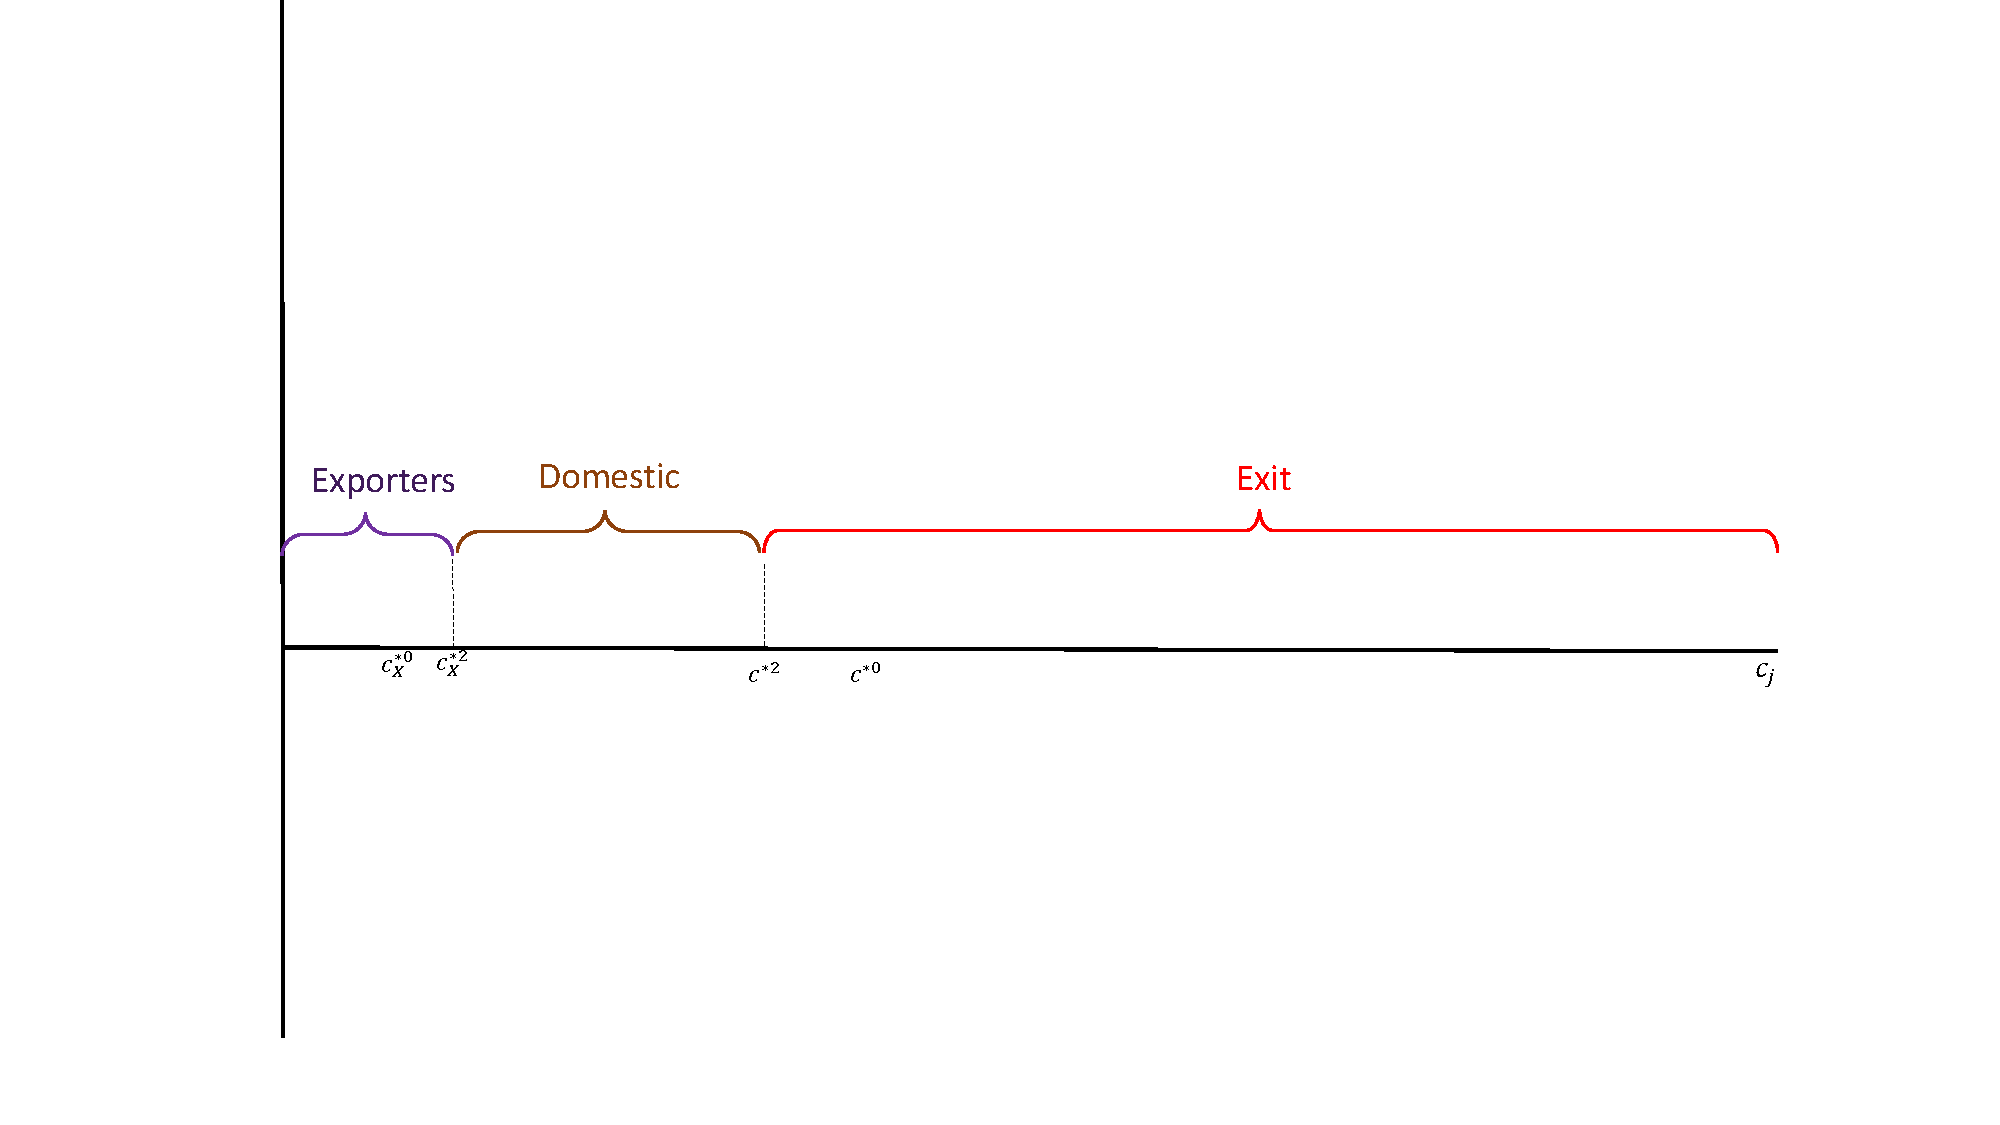
\includegraphics[scale=0.32]{SL4_30.pdf}
	
\end{frame}

\begin{frame}
	\frametitle{Trade liberalization with heterogeneous firms and fixed export costs: Conclusion}
		\begin{itemize}
			\item Highest cost firms are forced out of the market.
			\item More firms select into exporting.
				\begin{itemize}
					\item At the margin, these are less productive (higher cost) firms. 
				\end{itemize}
			\item Consumers still enjoy variety gains ($n\uparrow$)
			\item Allocative gains from trade due to exit of highest cost firms.

		\end{itemize}
	
\end{frame}

\section{Empirics}

\subsection{Trefler 2004}

\begin{frame}
	\frametitle{Trefler (2004): Effect of Canada U.S. FTA on productivity}


\begin{itemize}
	\item While NAFTA went into force in 1993, the Canadian-American Free Trade Agreement (FTA) was enacted in 1989.
	\item Involved tariff concessions by both Canada and the United States.
	\item Prior to this one in four Canadian industries were protected by average stated tariffs of at least 10\%.
	\item Canadian firms were protected by average tariffs of 8.1\% with an average effective tariff of 16.1\%.
\end{itemize}
\end{frame}


\begin{frame}
	\frametitle{We have talked a lot about gains- what about loses?}
\begin{itemize}
	\item Canadian manufacturing fell by 5\% (100,000 jobs!) following implementation of the FTA.
	\begin{itemize}
		\item What is the counterfactual? Unclear.
	\end{itemize}
	\item Short-run labour adjustment costs due to trade liberalization
		\begin{itemize}
			\item However, within ten years, employment rates had recovered.
				\begin{itemize}
					\item Gains are generally a long-run phenomenon. 
				\end{itemize}
		\end{itemize}
\end{itemize}
\end{frame}

\begin{frame}
	\frametitle{Main findings of Trefler (2004):}

\begin{itemize}
	\item The least productive firms in the contracted/suffered in Canadian sectors that benefited from tariff cuts. \\
	\begin{itemize}
		\item Explicitly predicted by the above model as the most productive firms enhance their productive scale.
	\end{itemize}

	\item In formerly sheltered industries, labour productivity (value added per worker) grew by 15\%.
	\begin{itemize}
		\item Approximately half came from reallocation across firms and the remainder from \emph{within} firm improvements.
		\item Firm heterogeneity model explains the first half.
		\begin{itemize}
			\item What explains within-firm improvements?
		\end{itemize}
	\end{itemize}
	\item Tradeoff: Employment fell in these industries by 12\%.
		\begin{itemize}
			\item Do the long-run productivity benefits outweigh the short-run costs?
		\end{itemize}
	\end{itemize}

\end{frame}

\subsection{Lileeva and Trefler 2010}

\begin{frame}
	\frametitle{Lileeva and Trefler (2010)}

Further examination of the ``within-firm" productivity improvements surrounding the FTA.
\begin{itemize}
	\item "Improved Access to Foreign Markets Raises Plant Level Productivity... For Some Plants."
	\item Examines whether access to foreign markets encourages firms to \emph{invest} in productivity improvements.
		\begin{itemize}
			\item Use plants specific tariff cuts to disentangle this effect.
		\end{itemize}
\end{itemize}
\end{frame}

\begin{frame}
	\frametitle{Lileeva and Trefler (2010): Main Findings}
	
	\begin{itemize}
		\item Magnitude of different productivity gains in manufacturing:
			\begin{itemize}
				\item Exit of least productive plants increased average productivity by 4.3 \%
				\item Increased market share of exporters raised average productivity by 4.1\%
				\item Within-firm productivity improvements increased average productivity by 4.8-5.6\%
		\end{itemize}
	\end{itemize}
\end{frame}

\begin{frame}
	\frametitle{Lileeva and Trefler (2010): Evidence on Mechanisms}
Provide further evidence on the within-firm productivity improvements. 
				\begin{itemize}
					\item Theory: 
						\begin{itemize}
							\item If productivity improvements driven by incentives to invest, lower productivity firms that begin exporting for the first time will have the highest incentives to invest in productivity improvements.
							\item Roughly, these firms need to ``catch up" the most if they want to compete in world markets!
						\end{itemize}
					\item We see the largest productivity gains for the least productive firms that entered the export market. 
					\item Using survey data, also find that least productive, new exporters, were the most likely to adopt new technologies. 
				\end{itemize}
\end{frame}



\section{External Economies of Scale (KOM Ch. 7)}

\subsection{Introduction}

\begin{frame}
	\frametitle{Motivation: Industrial Clusters}
Many industries tend to concentrate in a single location:
\begin{itemize}
	\item Some well-known examples:
	\begin{itemize}
		\item Silicon Valley
		\item Hollywood
		\item Investment banking in New York
	\end{itemize}
	\item Why does this happen?
\end{itemize}
\end{frame}

\begin{frame}
	\frametitle{External Economies of Scale}
	Alfred Marshall argued that industrial clusters tend to occur in industries characterized by \emph{external} economies of scale.
	\begin{itemize}
		\item \textbf{External economies of scale}: Average costs fall as the output of \underline{the industry} increases.
			\begin{itemize}
				\item Basic Idea: If being located near other firms generates ``positive spillovers," average cost may fall as more and more firms enter the same area.
				\item Key difference relative to internal economies of scale:
					\begin{itemize}
						\item Each firm takes industry scale (or industry average costs) as \emph{exogenous}.
					\end{itemize}
			\end{itemize}
	\end{itemize}
	
\end{frame}

\begin{frame}
	\frametitle{Sources of Extrernal Economies of Scale}
	
	What generates external economies of scale? \vspace{3mm}
		\begin{enumerate}
			\item Specialized suppliers
			\item Labour market pooling
			\item Knowledge spillovers
		\end{enumerate}\vspace{5mm}
	Let's consider each of these in turn.\vspace{3mm}

\end{frame}
\begin{frame}
	\frametitle{Specialized Suppliers}
\begin{itemize}
	\item Many industries require require inputs that are highly specialized inputs.
		\begin{itemize}
			\item E.g. semiconducters and computer chips.
		\end{itemize}
	\item Problem: Firms may not wish to specialize in producing highly specialized inputs if market size is too small.
		\begin{itemize}
			\item Could always produce inputs internally, but loss in efficiency
		\end{itemize}
	\item Solution: If many ``downstream" firms locate in the same area, generates a large enough market size for independent input suppliers to be viable (the ``upstream" firms).
		\begin{itemize}
			\item Note gains due to specialized suppliers will tend to generate ``path dependence."
				\begin{itemize}
					\item Once some input suppliers start to locate in the same area (which could be anywhere!), very little incentive for downstream firms to locate anywhere else!
				\end{itemize}
		\end{itemize}.
\end{itemize}
	
\end{frame}

\begin{frame}
	\frametitle{Specialized Suppliers}

		\emph{``...engineers left established semiconductor companies to start firms that manufactured capitals goods such as diffusion ovens, step-and-repeat cameras, and testers, and materials and components such as photomasks, testing jigs, and specialized chemicals.... This independent equipment sector promoted the continuing formation of semiconductor firms by freeing individual producers from the expense of developing capital equipment internally and by spreading the costs of development. It also reinforced the tendency towards industrial localization, as most the specialized inputs were not available elsewhere in the country. "} 
		
		\vspace{3mm}(On specialized suppliers in Silicon Valley, quoted in KOM Ch. 7)
	
\end{frame}


\begin{frame}
	\frametitle{Labor Market Pooling}
Similar to specialized suppliers, except applied to a particular factor, \emph{labour}.
	\begin{itemize}
		\item Some jobs require highly specialized skills.
			\begin{itemize}
				\item Film animation or special effects production.
			\end{itemize}
		\item Workers with highly specialized skills are going to want to locate in regions with lots of potential employers.
			\begin{itemize}
				\item Easier to find/change jobs.
			\end{itemize}
		\item Firms also want to locate in regions with lots of potential employees
			\begin{itemize}
				\item Less likely to have to deal with labour shortages.
			\end{itemize}
		\item These gains are very important when demand is highly uncertain.
	\end{itemize}
	
\end{frame}

\begin{frame}
	\frametitle{Labor Market Pooling: Example}
Consider a world with two film studios and 200 animators.
	\begin{itemize}
		\item Both studios face \emph{idiosyncratic} demand uncertainty:
			\begin{itemize}
				\item If studio-level demand is high, will want hire 150 workers.
				\item If demand is low, will only want to hire 50 workers.
			\end{itemize}
		\item Let's consider what happens if the studios locate in different cities, and when they locate in the same city
	\end{itemize}


\end{frame}

\begin{frame}
	\frametitle{Labour Market Pooling: Example}
Suppose both studios locate in different cities.
			\begin{itemize}
				\item Suppose 100 animators go to each city.
				\item If demand is high for either firm, there is a labour shortage!
				\item If demand is low for either firm, some animators are unemployed!
			\end{itemize}
At least one side of the market is hurt no matter what!
\end{frame}

\begin{frame}
	\frametitle{Labour Market Pooling: Example}
	Suppose both studios locate in the same cities.
	\begin{itemize}
		\item All animators are now located in the same place as well.
		\item There will only be labour shortage if demand is high for \emph{both} firms!
		\item Similarly, there will only be unemployment if demand if low for both firms. 
		\item Whenever one firm has high demand, and the other has low demand, the market clears.
	\end{itemize}
	This environment is much less risky. 

\end{frame}

\begin{frame}
	\frametitle{Labour Market Pooling: Silicon Valley}

		\emph{``...it wasn't a big catastrophe if you quit your job on Friday and have another job on Monday... You didn't necessarily have to tell your wife. You just drove off in another direction on Monday morning."} (Silicon Valley engineer)
	
\end{frame}

\begin{frame}
	\frametitle{Knowledge Spillovers}
To remain competitive highly innovative industries, it is crucial that one remain near the ``technology frontier."
	\begin{itemize}
		\item People like to talk about what they do.
			\begin{itemize}
				\item Informal exchange of ideas by employees after-hours may help keep one's firm up to date.
			\end{itemize} 
	\end{itemize}
	

		\emph{``Every year there was some place, the Wagon Wheel, Chez Yvonne, Rickey's, the Roundhouse, where members of this esoteric fraternity, the young men and women of the semiconductor industry, would head after work to have a drink and gossip and trade war stories about phase-jitters, phantom circuits, bubble memories, pulse trains, bounceless contracts, burst modes, leapfrog tests, p-n junctions, sleeping sickness modes, slow-death episodes, RAMs, NAKs, MOSes, PCMs, PROM blowers, PROM blasters, and teramagnitudes..."} (Tom Wolfe on early Silicon Valley)

	
\end{frame}

\subsection{Model}

\begin{frame}
	\frametitle{External Economies of Scale: Model}
We are going to consider a perfectly competitive model of external economies of scale.
	\begin{itemize}
		\item Partly for historical reasons
			\begin{itemize}
				\item External economies were first developed in this context
			\end{itemize}
		\item Partly for simplicity
			\begin{itemize}
				\item One ``type" of good, one price $\rightarrow$ much easier to solve
			\end{itemize}
	\end{itemize}
Basic environment:
	\begin{itemize}
		\item Large number of perfectly competitive and identical firms, each of whom supplies a negligible portion of industry output.
			\begin{itemize}
				\item Each firm takes industry output as given.	
			\end{itemize}
		\item Average costs fall with industry output.
		\item The economy is in a long-run equilibrium, so $P=AC$.
	\end{itemize}
	
\end{frame}

\begin{frame}
	\frametitle{External Economies of Scale Equilibrium}
		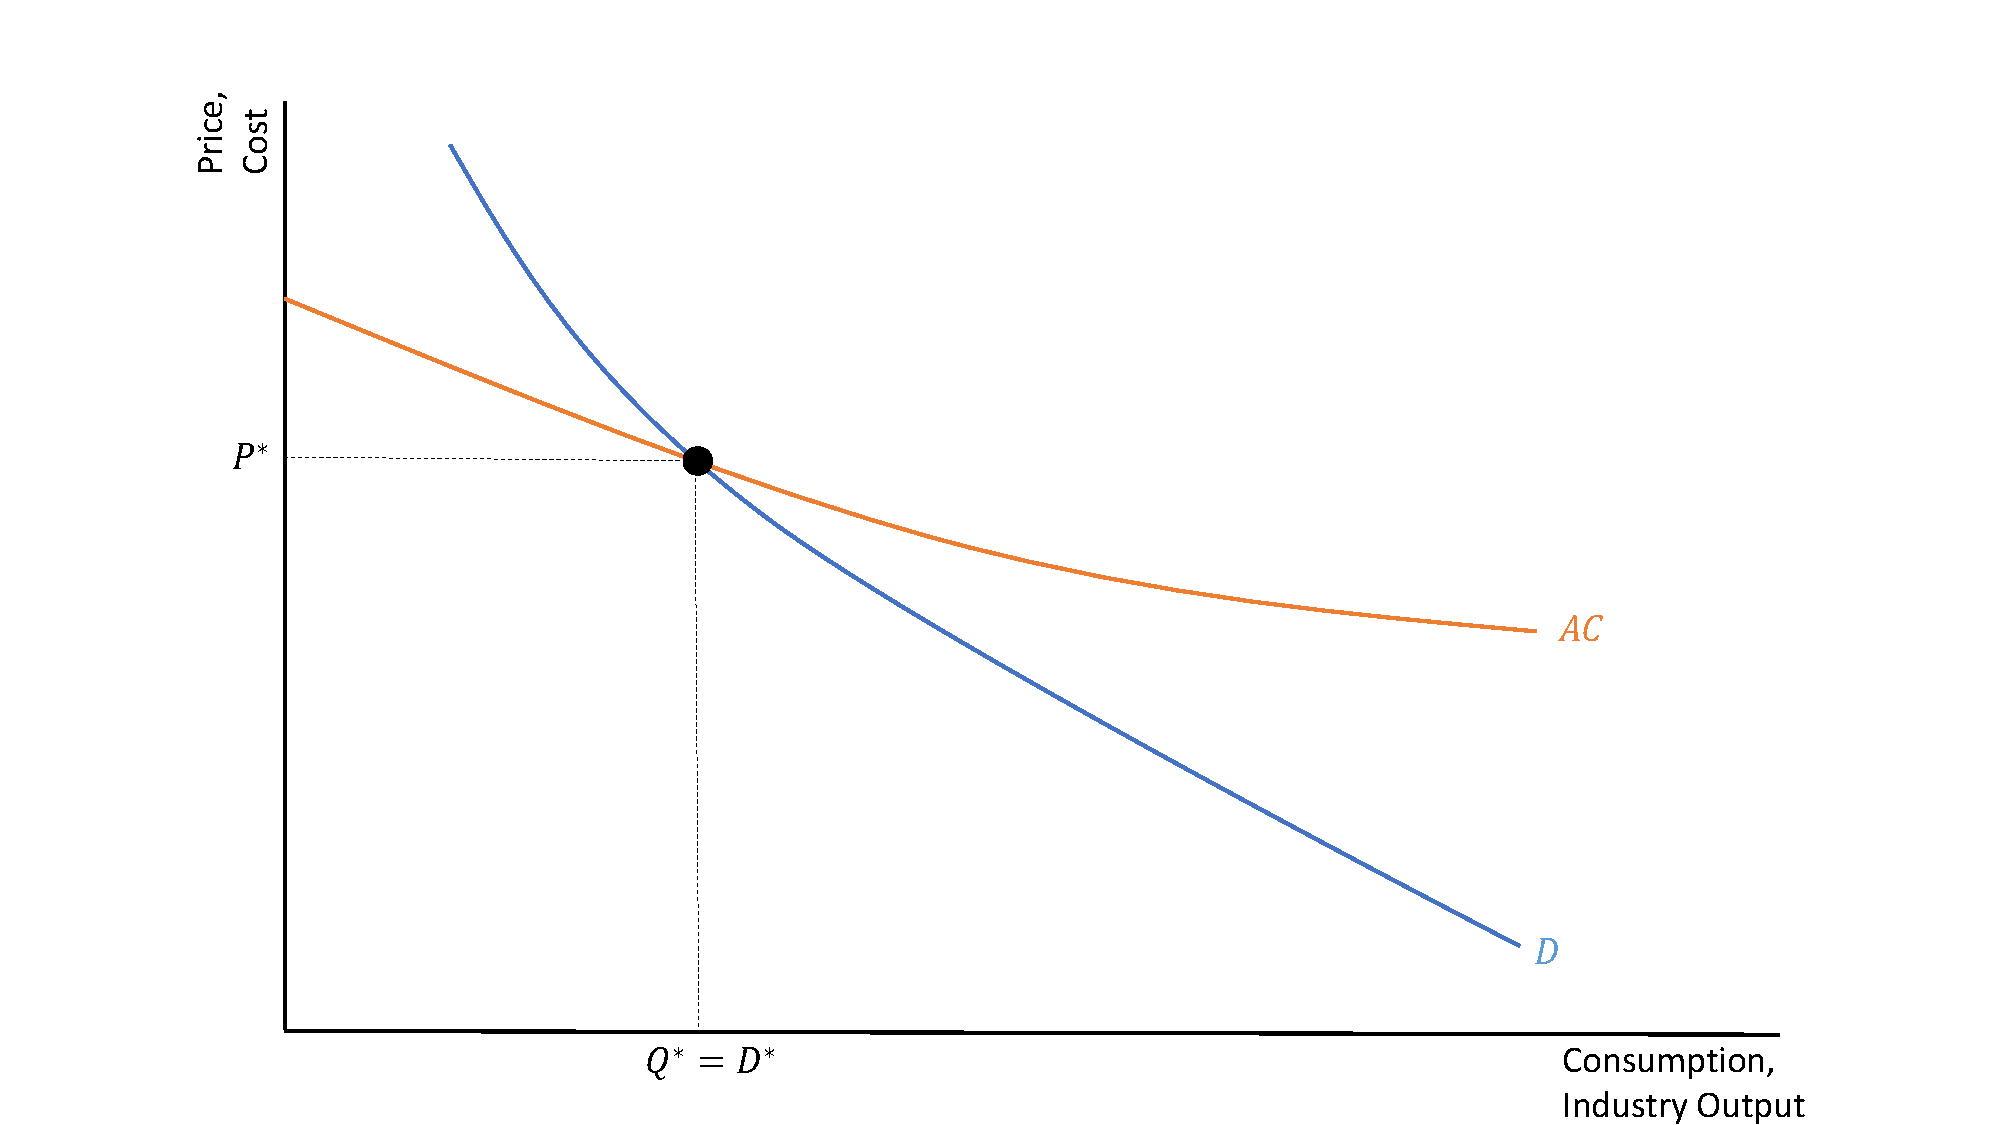
\includegraphics[scale=0.32]{SL4_17.pdf}
\end{frame}

\begin{frame}
	\frametitle{Trade and External Economies of Scale}
What happens in an environment with external economies and trade?
	\begin{itemize}
		\item Suppose Japan (JPN) and the United States (US)  have the \emph{exact same} inverse demand function for microchips, but different average cost curves.
			\begin{itemize}
				\item Let's suppose JPN has a cost advantage in microchip production $(AC_{JPN}<AC_{US})$
			\end{itemize}
		\item External returns to scale are ``local" in the sense that average costs fall with industry output \emph{within a country.}
			\begin{itemize}
				\item Higher output in Japan does not help the US, and \emph{vice versa}.
			\end{itemize}
	\end{itemize}
\end{frame}

\begin{frame}
	\frametitle{Autarky Equilibria}
	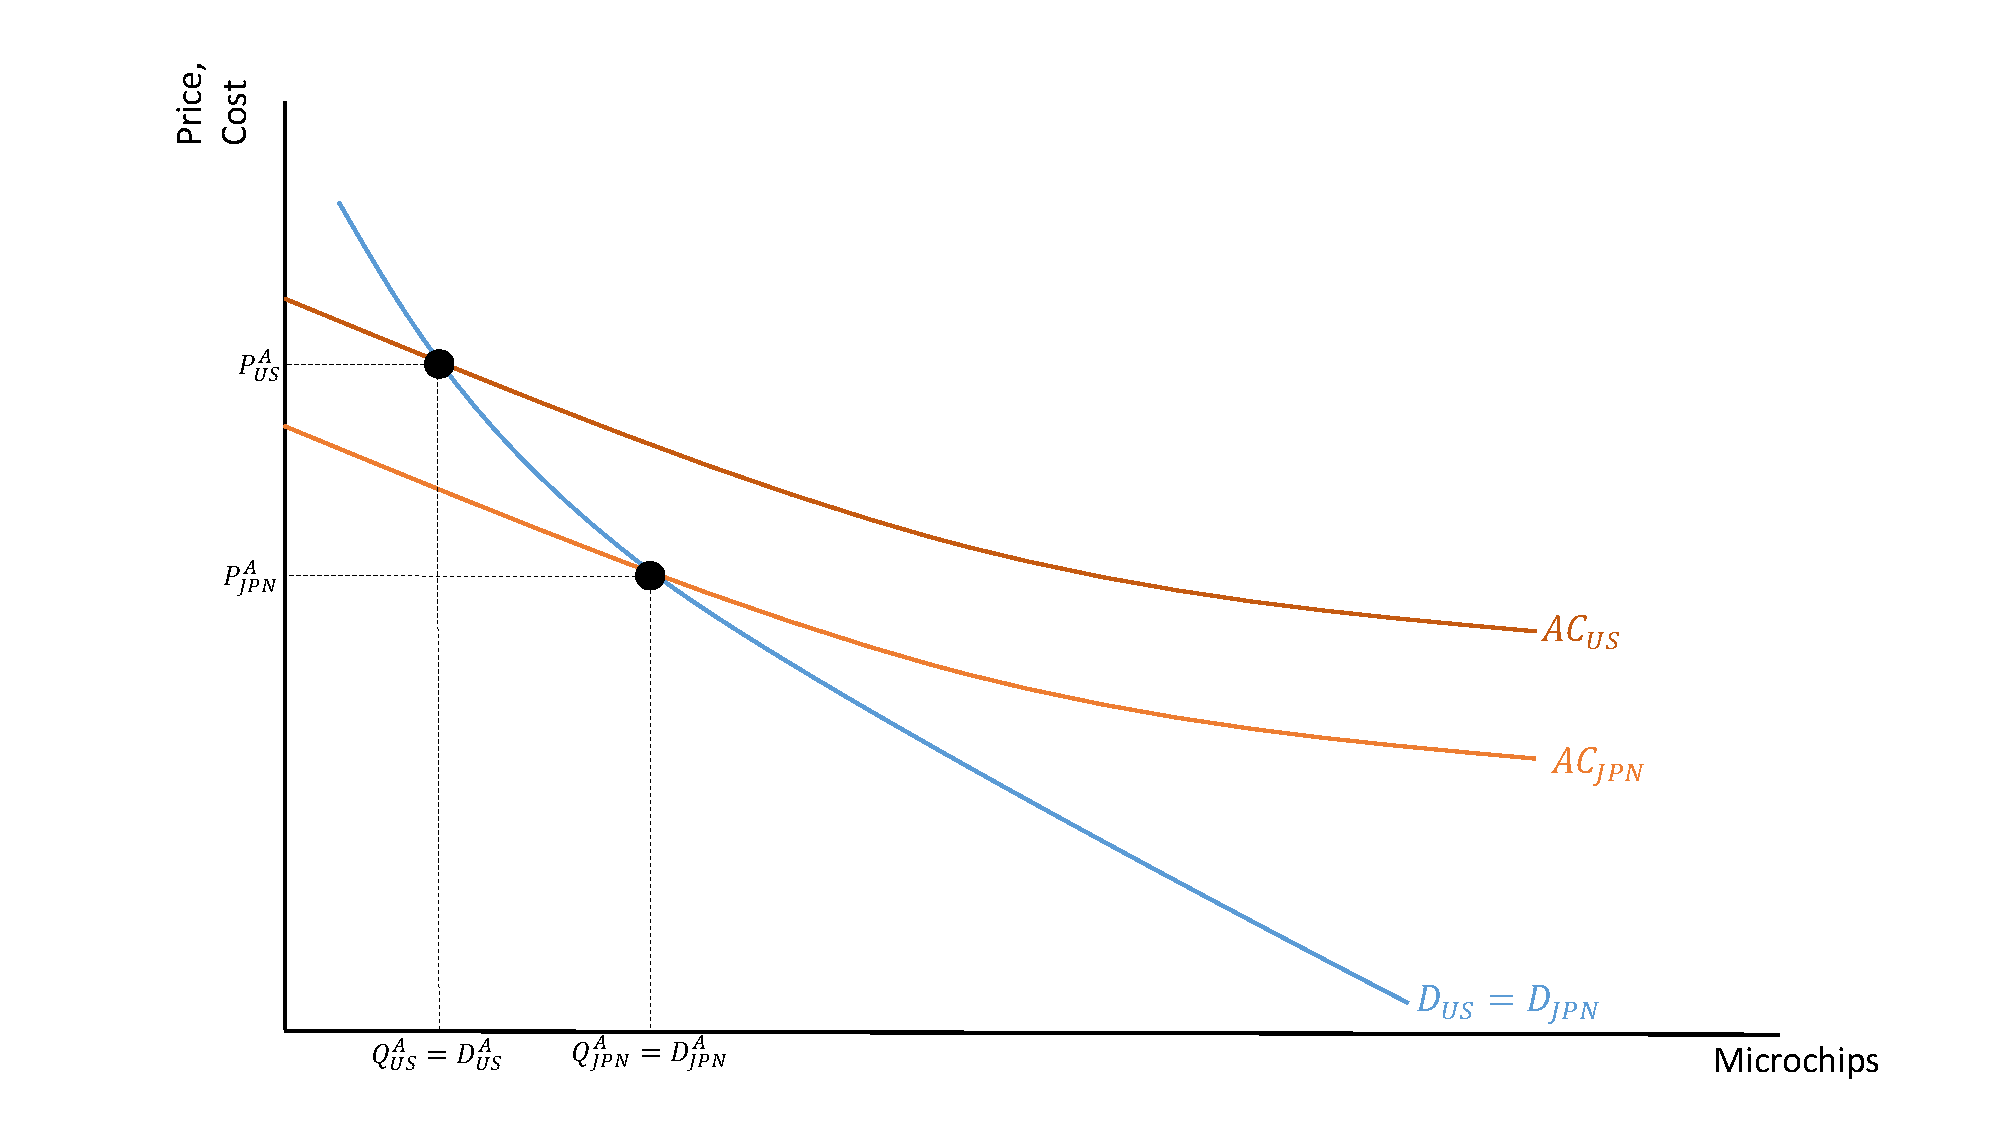
\includegraphics[scale=0.32]{SL4_18.pdf}
\end{frame}

\begin{frame}
	\frametitle{Opening up to trade with external economies of scale}
	\begin{itemize}
		\item Since $(P^A_{JPN}<P^A_{US})$, we should expect Japan to export microchips with free trade.
			\begin{itemize}
				\item With external economies, Japan takes over the whole market.
				\item Moreover, the new world price will lie \emph{below} both Japan and the US autarky price!
					\begin{itemize}
						\item Different prediction from standard comparative advantage models developed at the beginning of the course, where we would expect $P^A_{JPN}<P^T_{world}<P^A_{US}$ 
					\end{itemize}
			\end{itemize}
	\end{itemize}
\end{frame}

\begin{frame}
	\frametitle{Free Trade Equilibrium}
	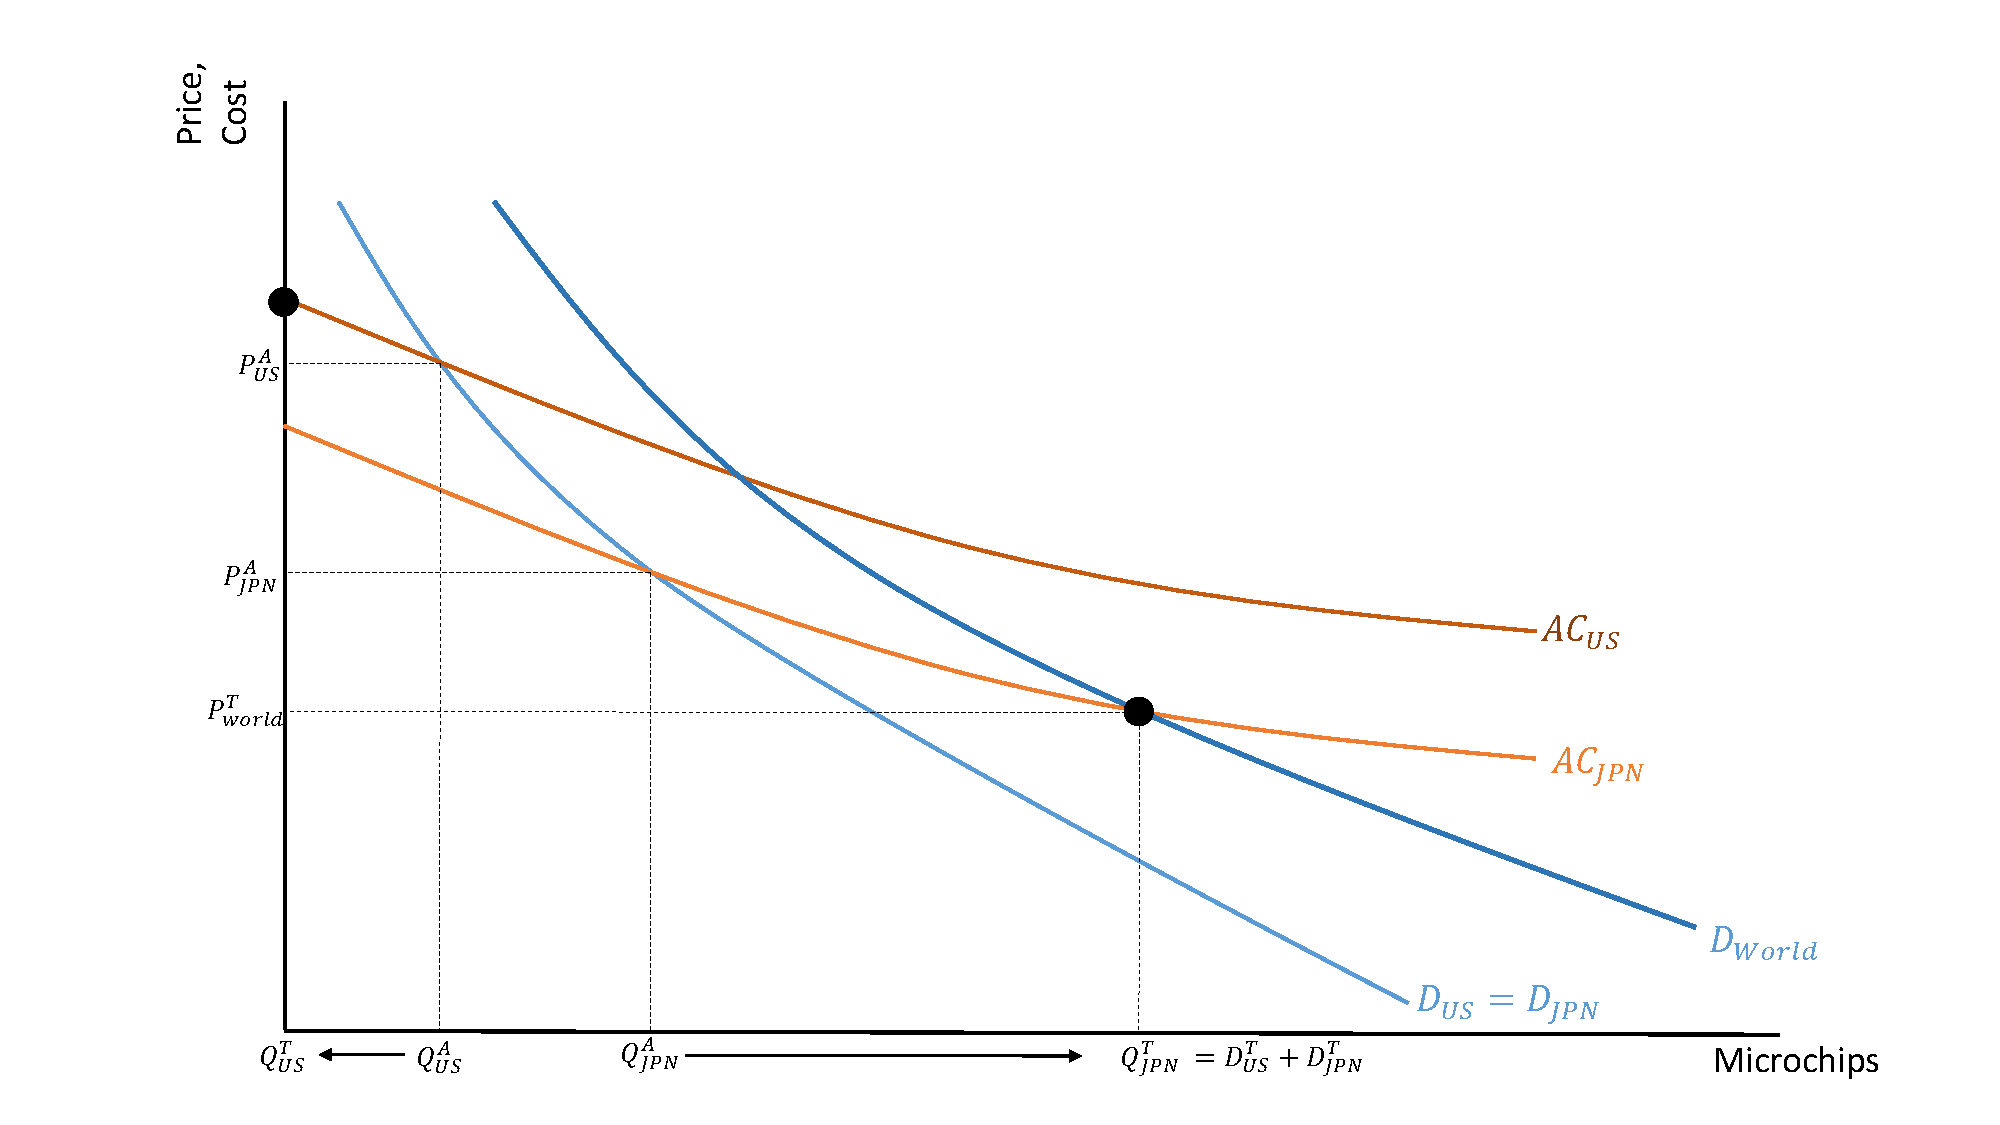
\includegraphics[scale=0.32]{SL4_19.pdf}
\end{frame}

\begin{frame}
	\frametitle{Gains from trade with external economies}
	\begin{itemize}
		\item Efficiency gains, 
			\begin{itemize}
				\item Increased Market Size $\rightarrow$ Cost savings due to (industry level) economies of scale.
			\end{itemize}
			
		\item  Consumer gains
			\begin{itemize}
				\item Price of microchips has fallen in both countries!
			\end{itemize}
	\end{itemize}
	Gains from trade look pretty good here!
\end{frame}

\begin{frame}
	\frametitle{Gains from trade with external economies}
...However
\begin{itemize}
	\item Models with external economies of scale \emph{do not} always imply that the right country will take over the industry!
		\begin{itemize}
			\item Due to the possibility of technological ``lock-in", a non-comparative advantage country could take over the entire market!
			\item To see this, suppose that the US had a much larger microchip market than Japan in Autarky.
		\end{itemize}
\end{itemize}
\end{frame}

\begin{frame}
	\frametitle{Autarky: Small Japanese market, large US market}
	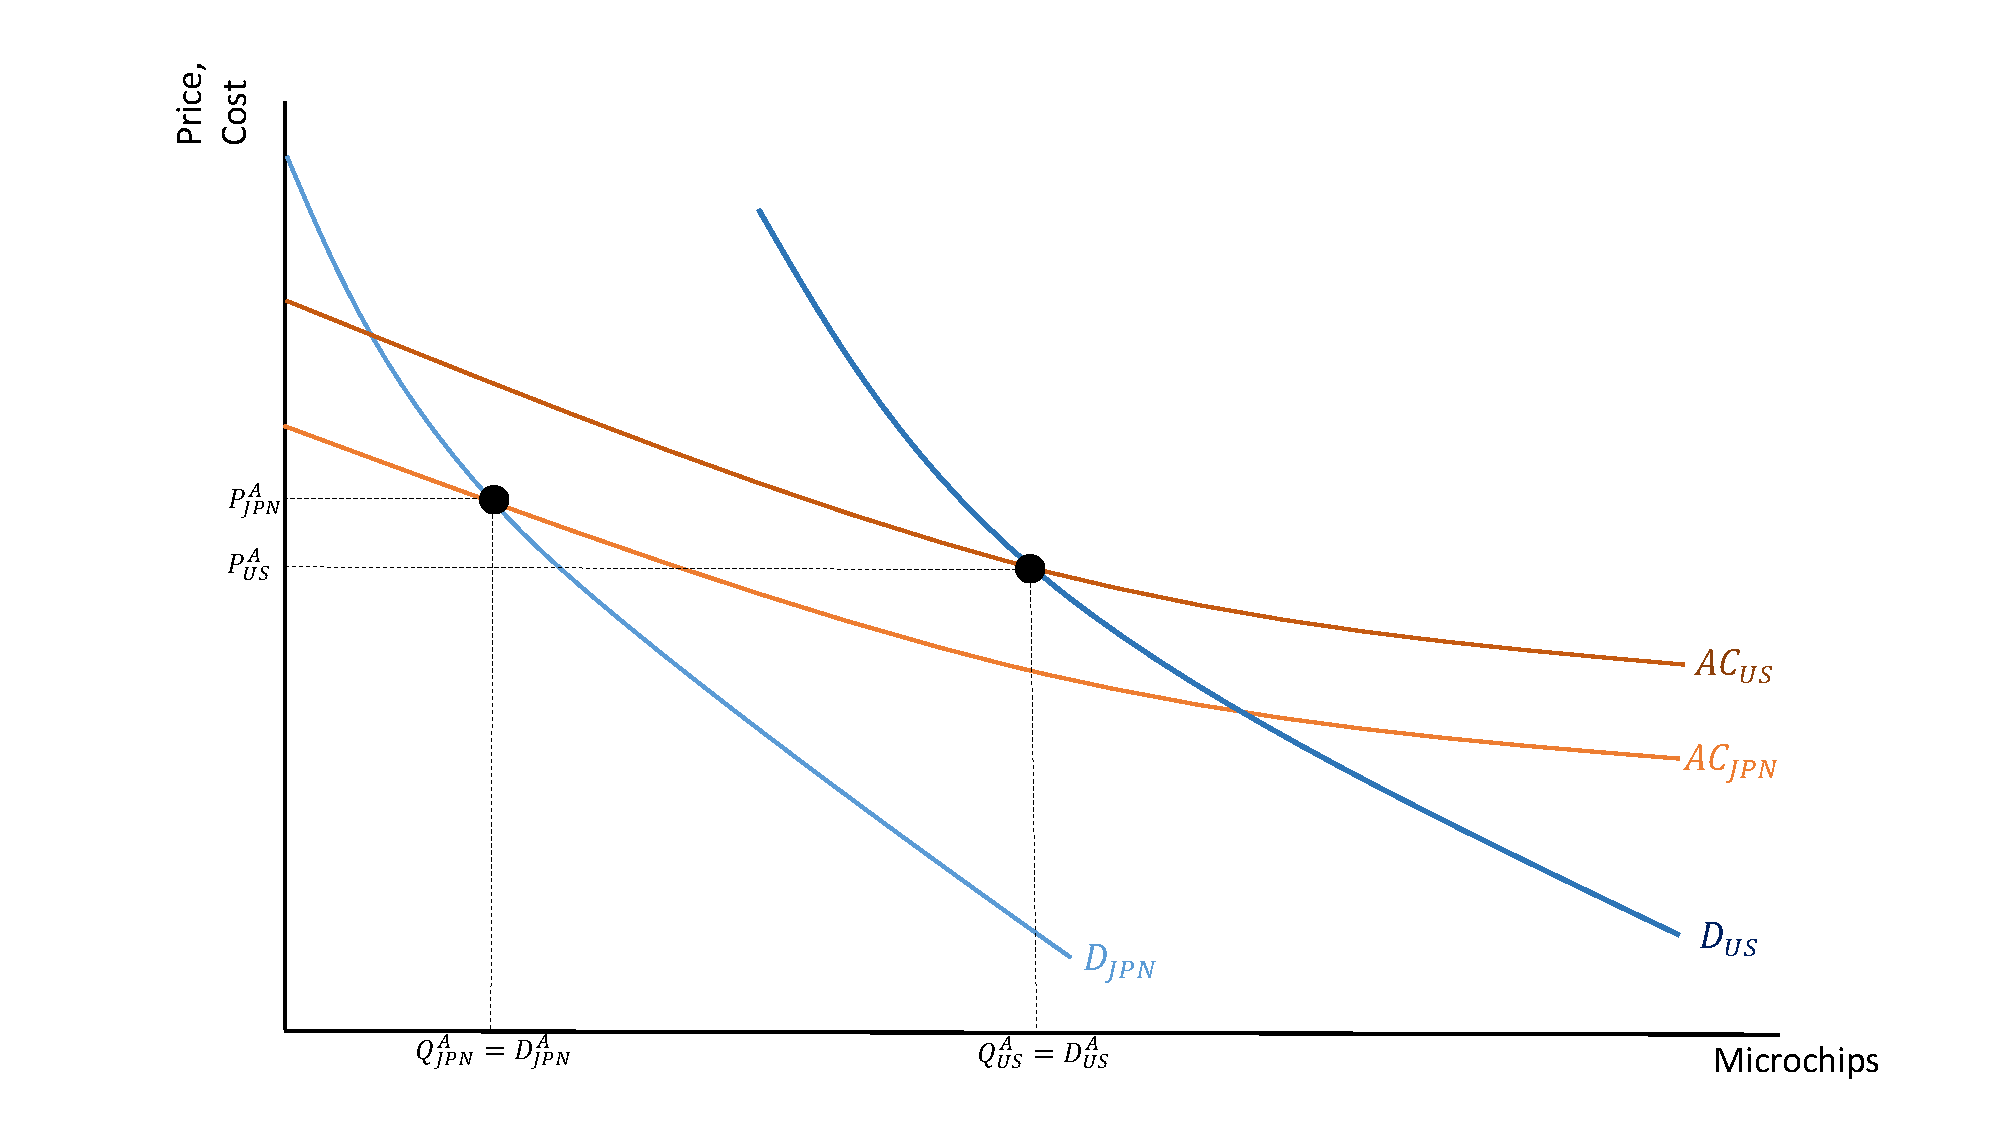
\includegraphics[scale=0.32]{SL4_20.pdf}
\end{frame}

\begin{frame}
	\frametitle{Trade: Small Japanese market, large US market}
	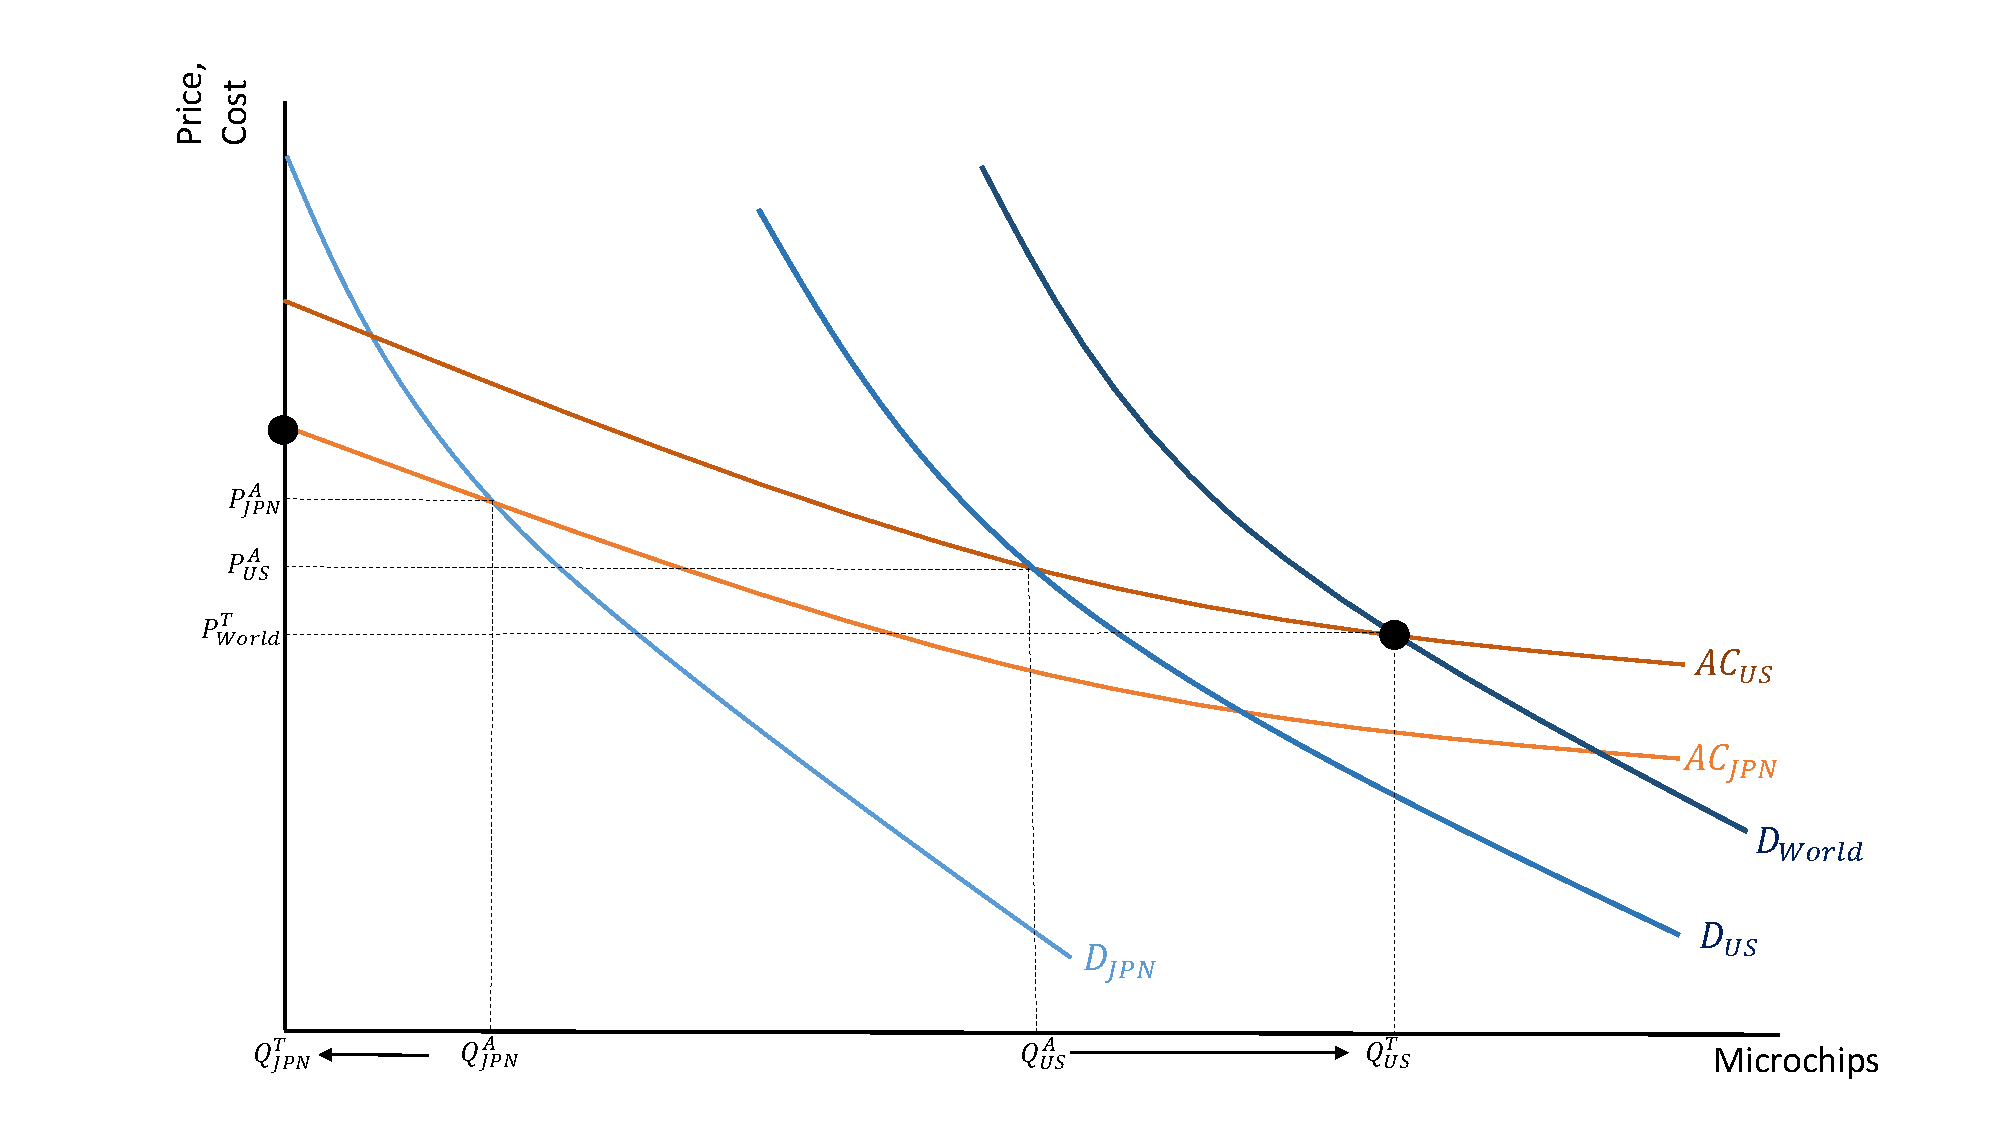
\includegraphics[scale=0.32]{SL4_21.pdf}
\end{frame}

\begin{frame}
	\frametitle{Trade: Small Japanese market, large US market}
	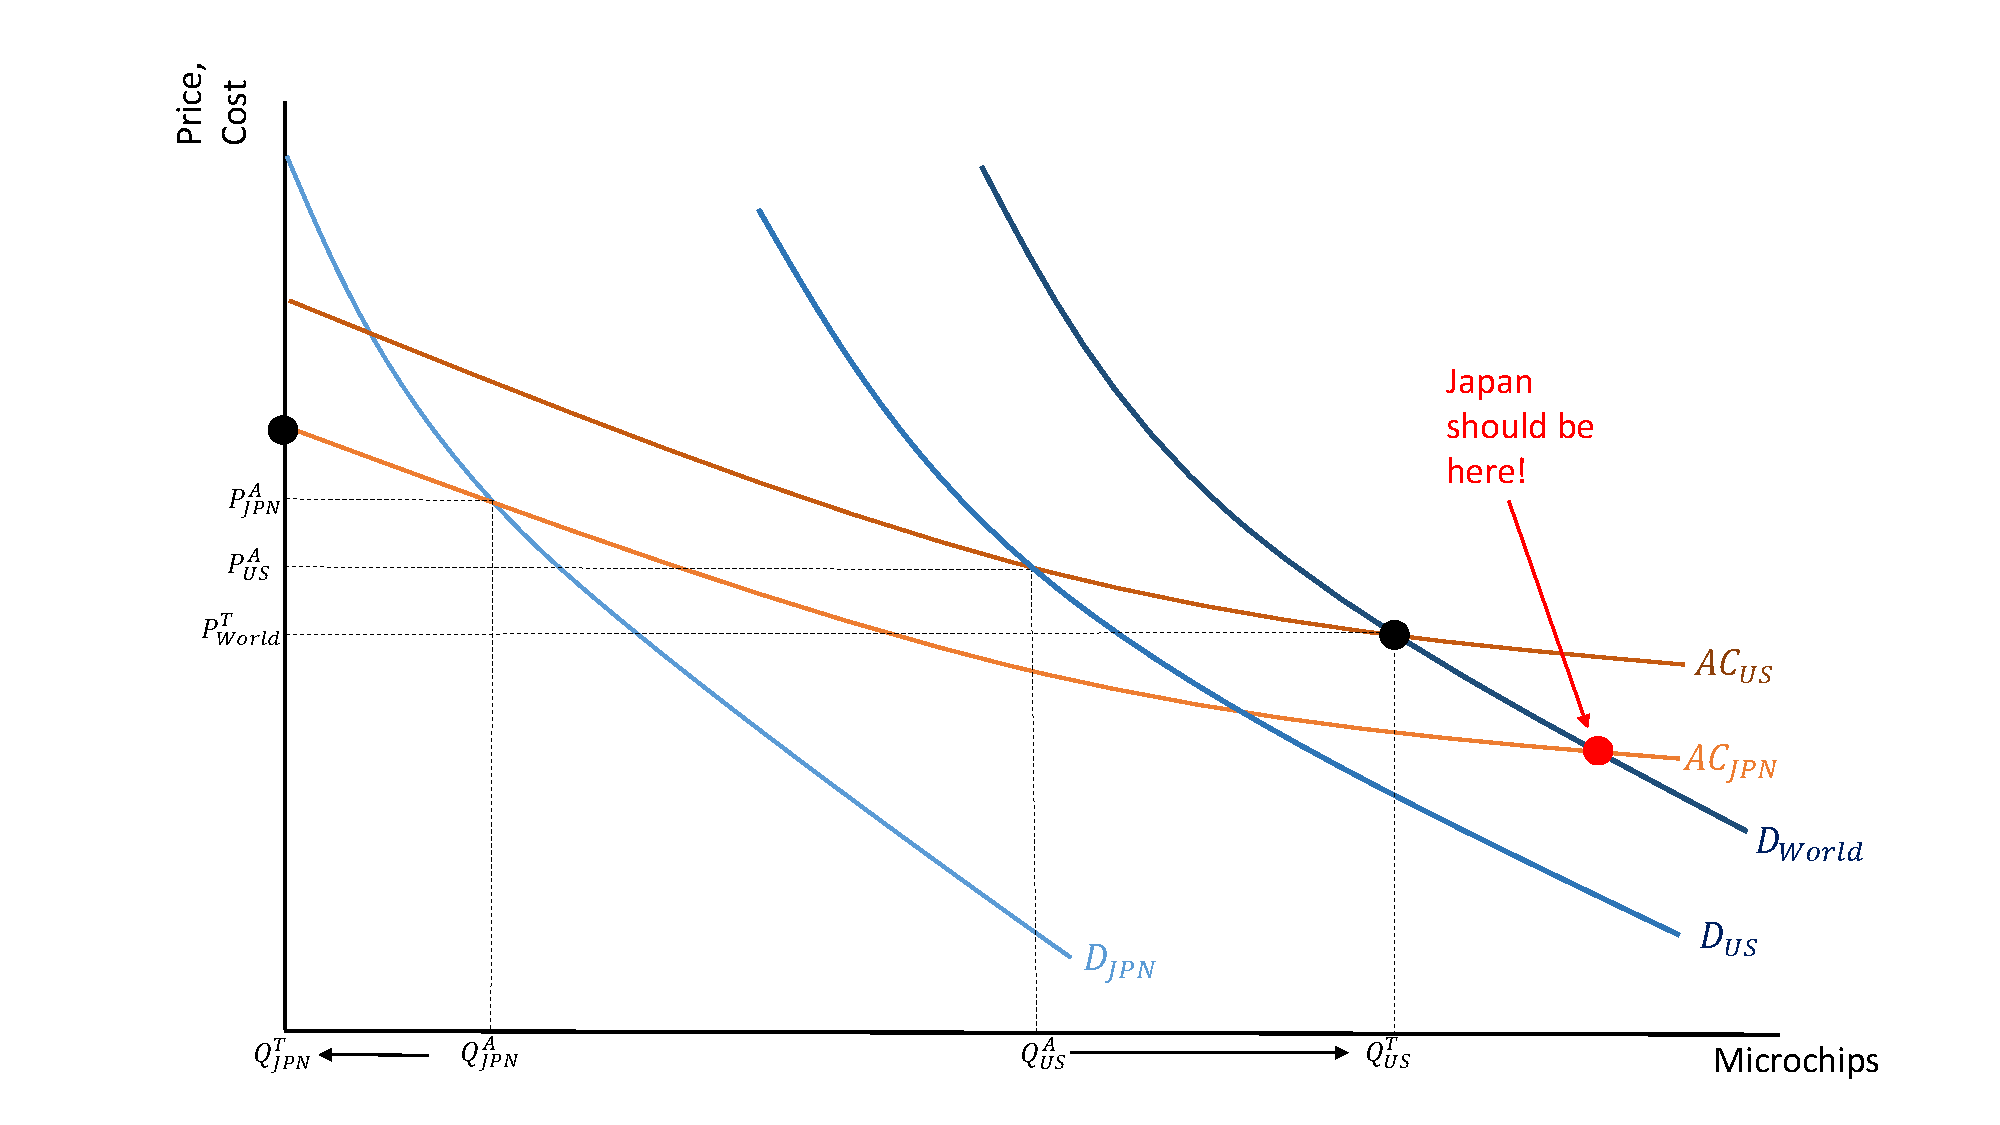
\includegraphics[scale=0.32]{SL4_22.pdf}
\end{frame}

\begin{frame}
	\frametitle{Trade: Small Japanese market, large US market}
	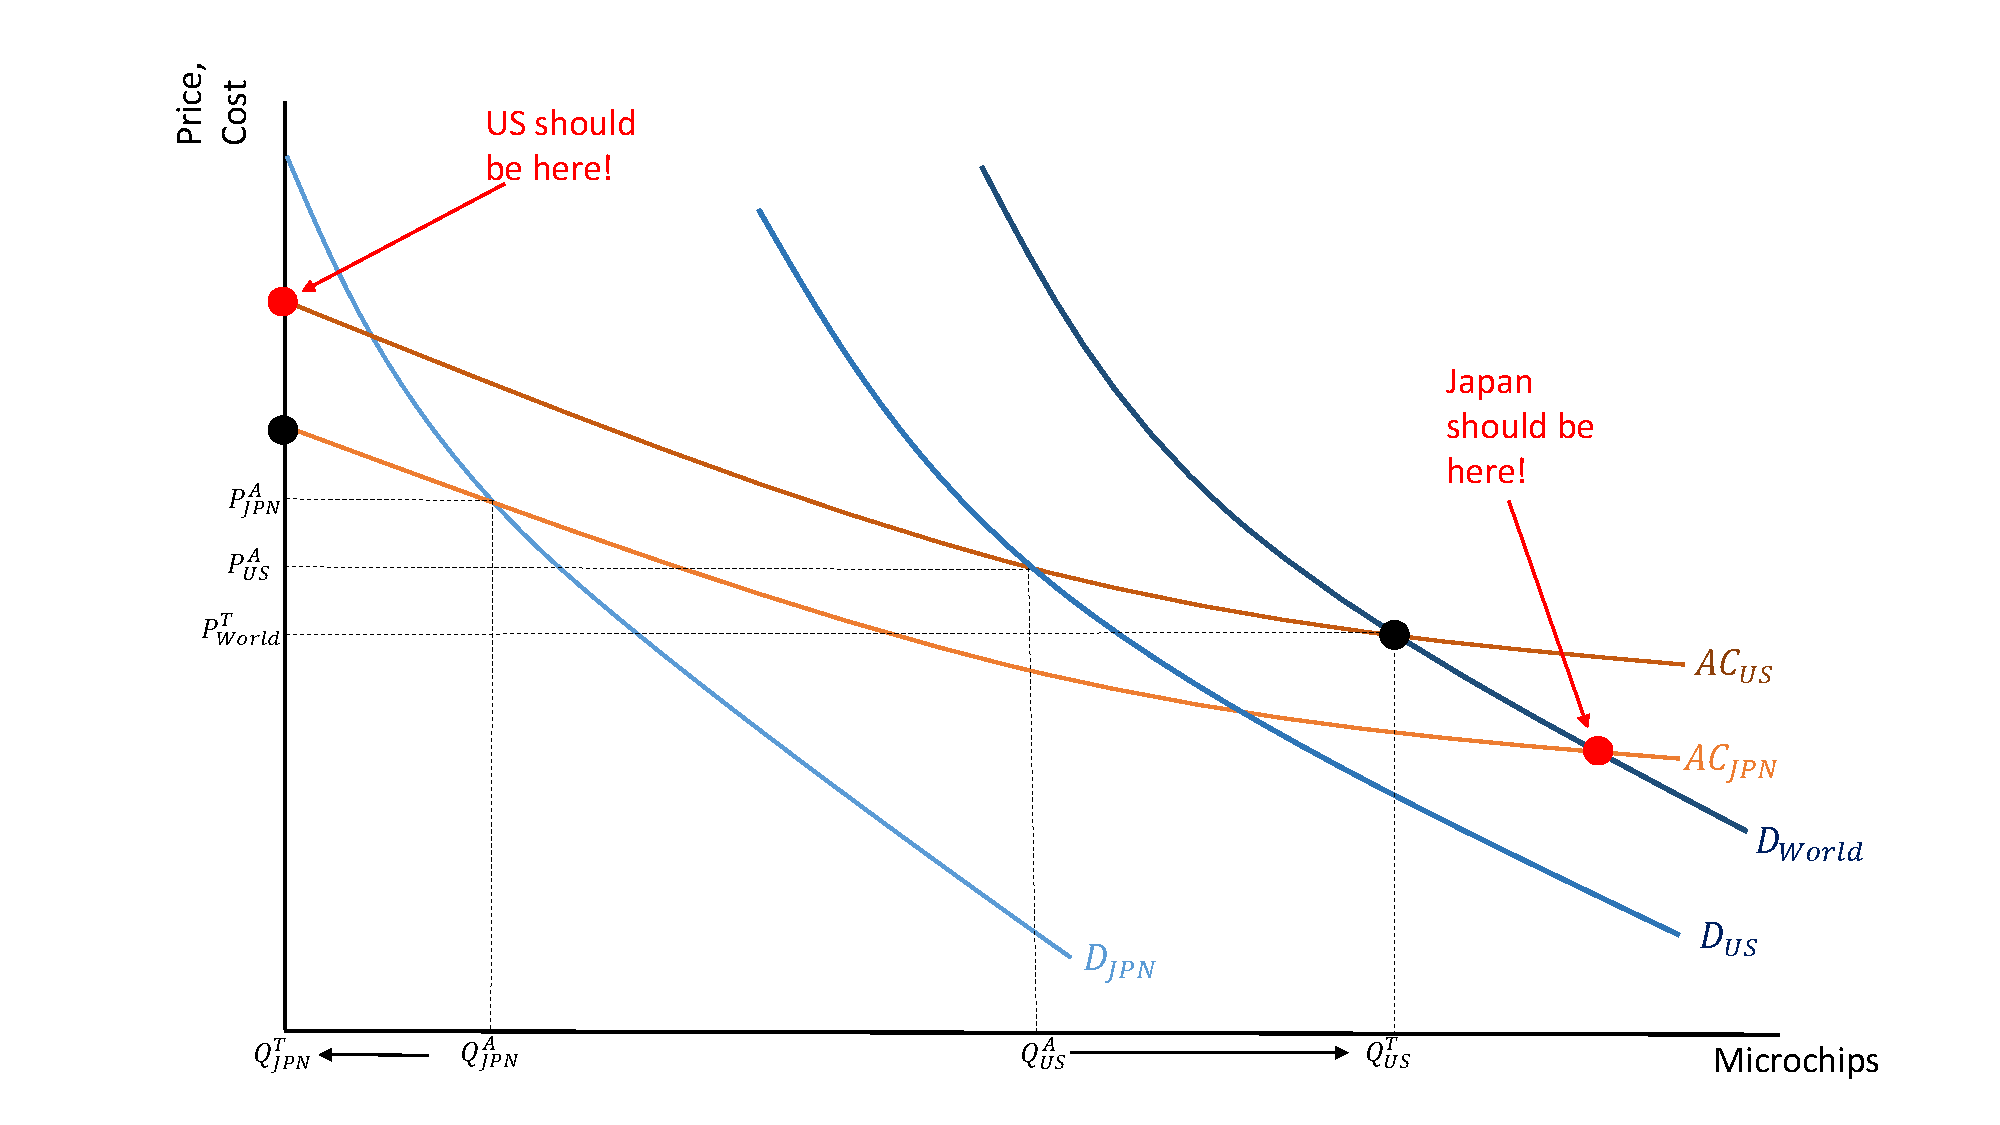
\includegraphics[scale=0.32]{SL4_23.pdf}
\end{frame}

\begin{frame}
	\frametitle{``Lock in" and the gains from trade}
	\begin{itemize}
		\item Since U.S. already had a larger microchip before opening up to trade, they take the whole world market.
			\begin{itemize}
				\item U.S. producers were able to price below Japanese producers average costs
				\item Japanese producers will not price that low since that will earn them negative profits.
				\item Nobody will buy from Japan if they price at their current (autarky) average cost.
					\begin{itemize}
						\item Industry output in Japan goes to zero, even though they ``should" take over the entire market!
					\end{itemize}
				\item We have smaller gains from trade then we ``could" have.
					\begin{itemize}
						\item Although there are still gains from trade. 
					\end{itemize}
			\end{itemize}
	\end{itemize}

\end{frame}

\subsection{Infant Industry Argument}

\begin{frame}
	\frametitle{``Infant industry" argument: A case for trade protection?}
Arguments based on the inefficiency of ``lock-in" are sometimes be used to justify limiting free trade.
	\begin{itemize}
		\item Trade protection may be warranted if:
			\begin{itemize}
				\item The low-cost country discovered the technology relatively late
				\item The low-cost country has sufficiently large demand for the industry. 
			\end{itemize}
		\item Let's consider a world where the U.S. discovered microchips first.
			\begin{itemize}
				\item Japan has yet to build a microchip industry, but has a natural cost advantage. 
			\end{itemize}
	\end{itemize}
\end{frame}

\begin{frame}
	\frametitle{Trade equilibrium with Japan as a ``new entrant"}
	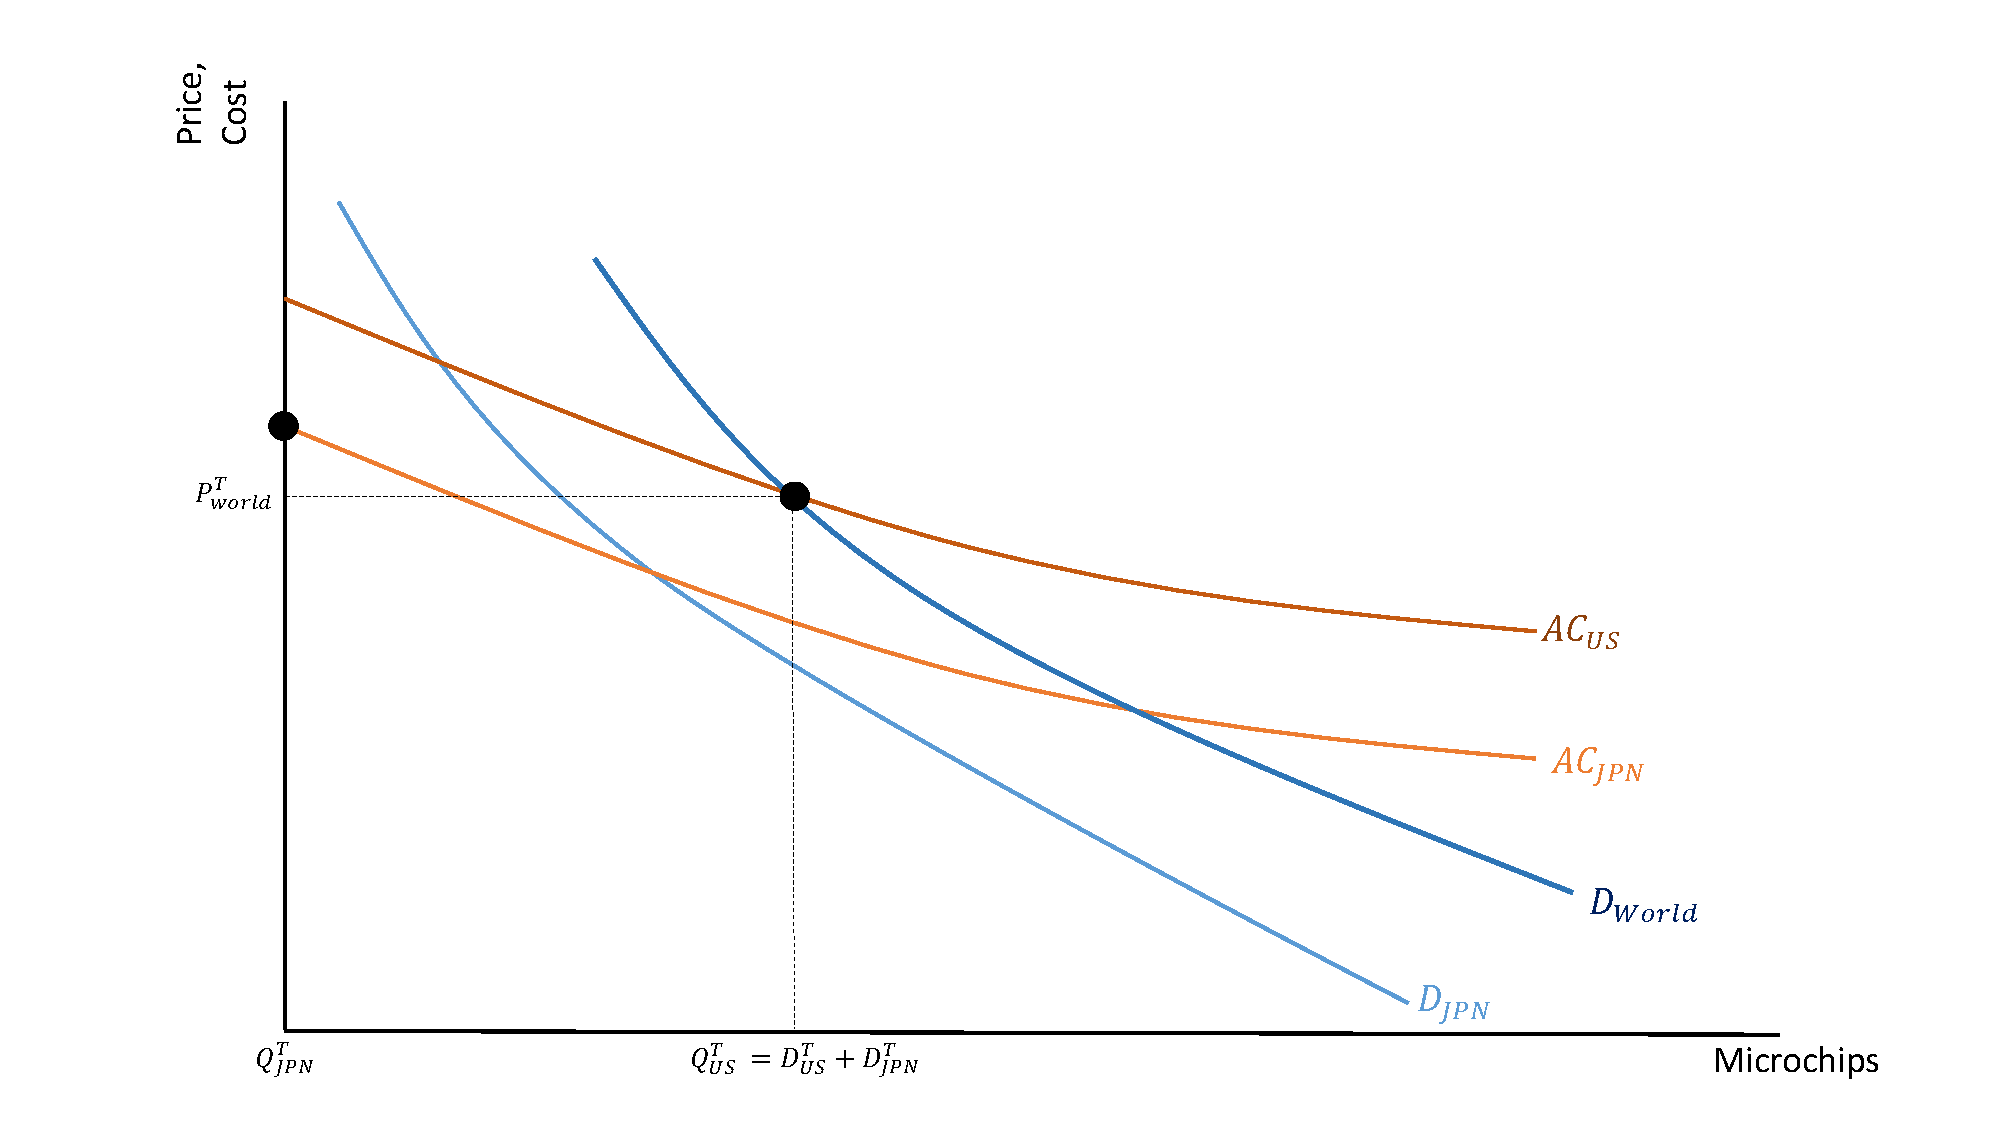
\includegraphics[scale=0.32]{SL4_24.pdf}
\end{frame}

\begin{frame}
	\frametitle{``Lock-in" and new entrants}
	\begin{itemize}
		\item Since Japan currently does not have a developed microchip industry, their US competitors can price below their (current) average costs.
			\begin{itemize}
				\item If Japan can shelter this industry from foreign competition, this may allow them to start moving down their average cost curve.
				\item Interestingly, Japan would be better of with autarky in this case.
			\end{itemize} 
	\end{itemize}
\end{frame}

\begin{frame}
	\frametitle{Gains from autarky?}
	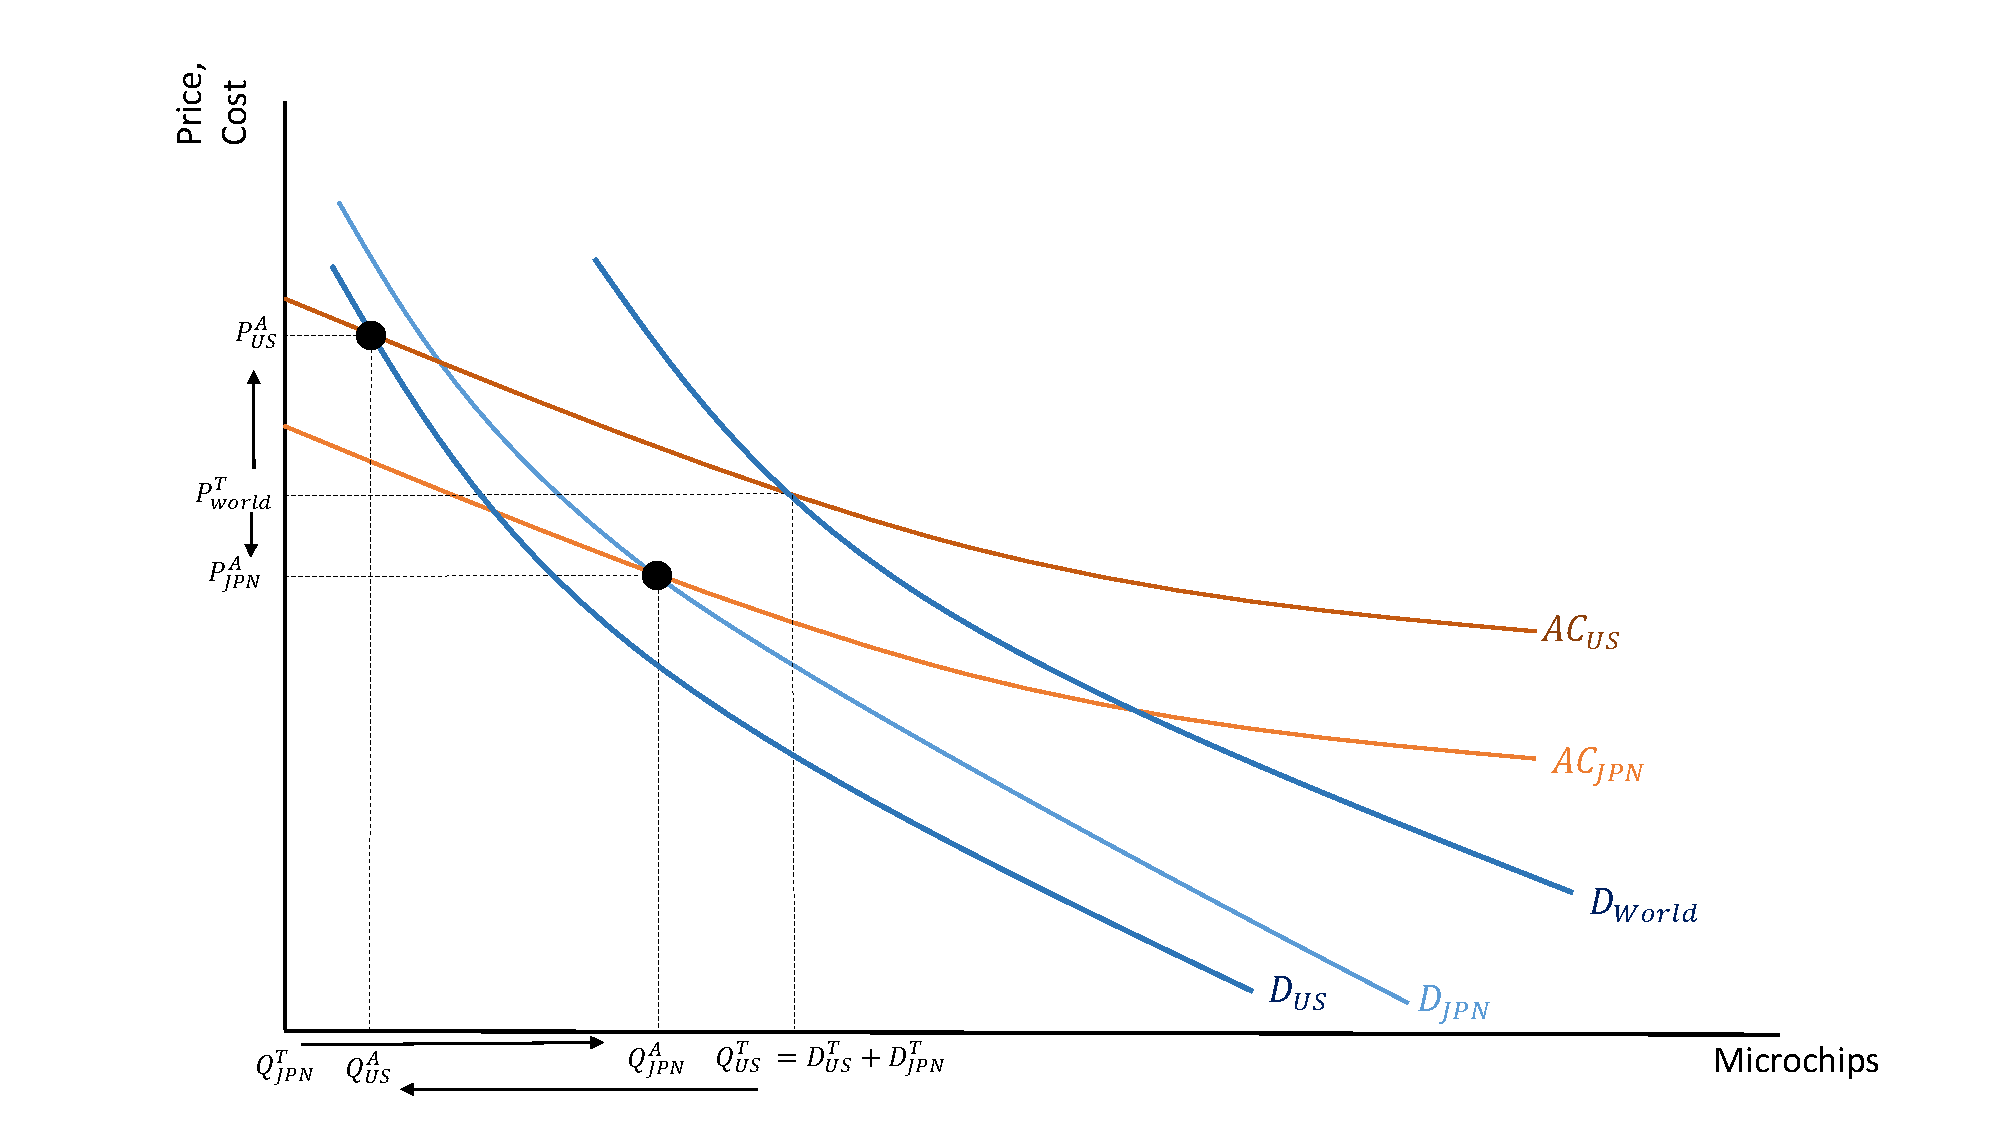
\includegraphics[scale=0.32]{SL4_25.pdf}
\end{frame}

\begin{frame}
	\frametitle{Eventual gains from trade?}
\begin{itemize}
	\item Japan is better of with autarky, compared to the free-trade equilibrium. 
	\item Note, however, that once they reached an autarky equilibrium, there are now gains from trade!
		\begin{itemize}
			\item Japan would now be able to out compete U.S. firms, and take over the entire market.	
			\item This would allow them to move even further down their average cost curve. 
		\end{itemize}
\end{itemize}
\end{frame}

\begin{frame}
	\frametitle{Eventual gains from trade}
	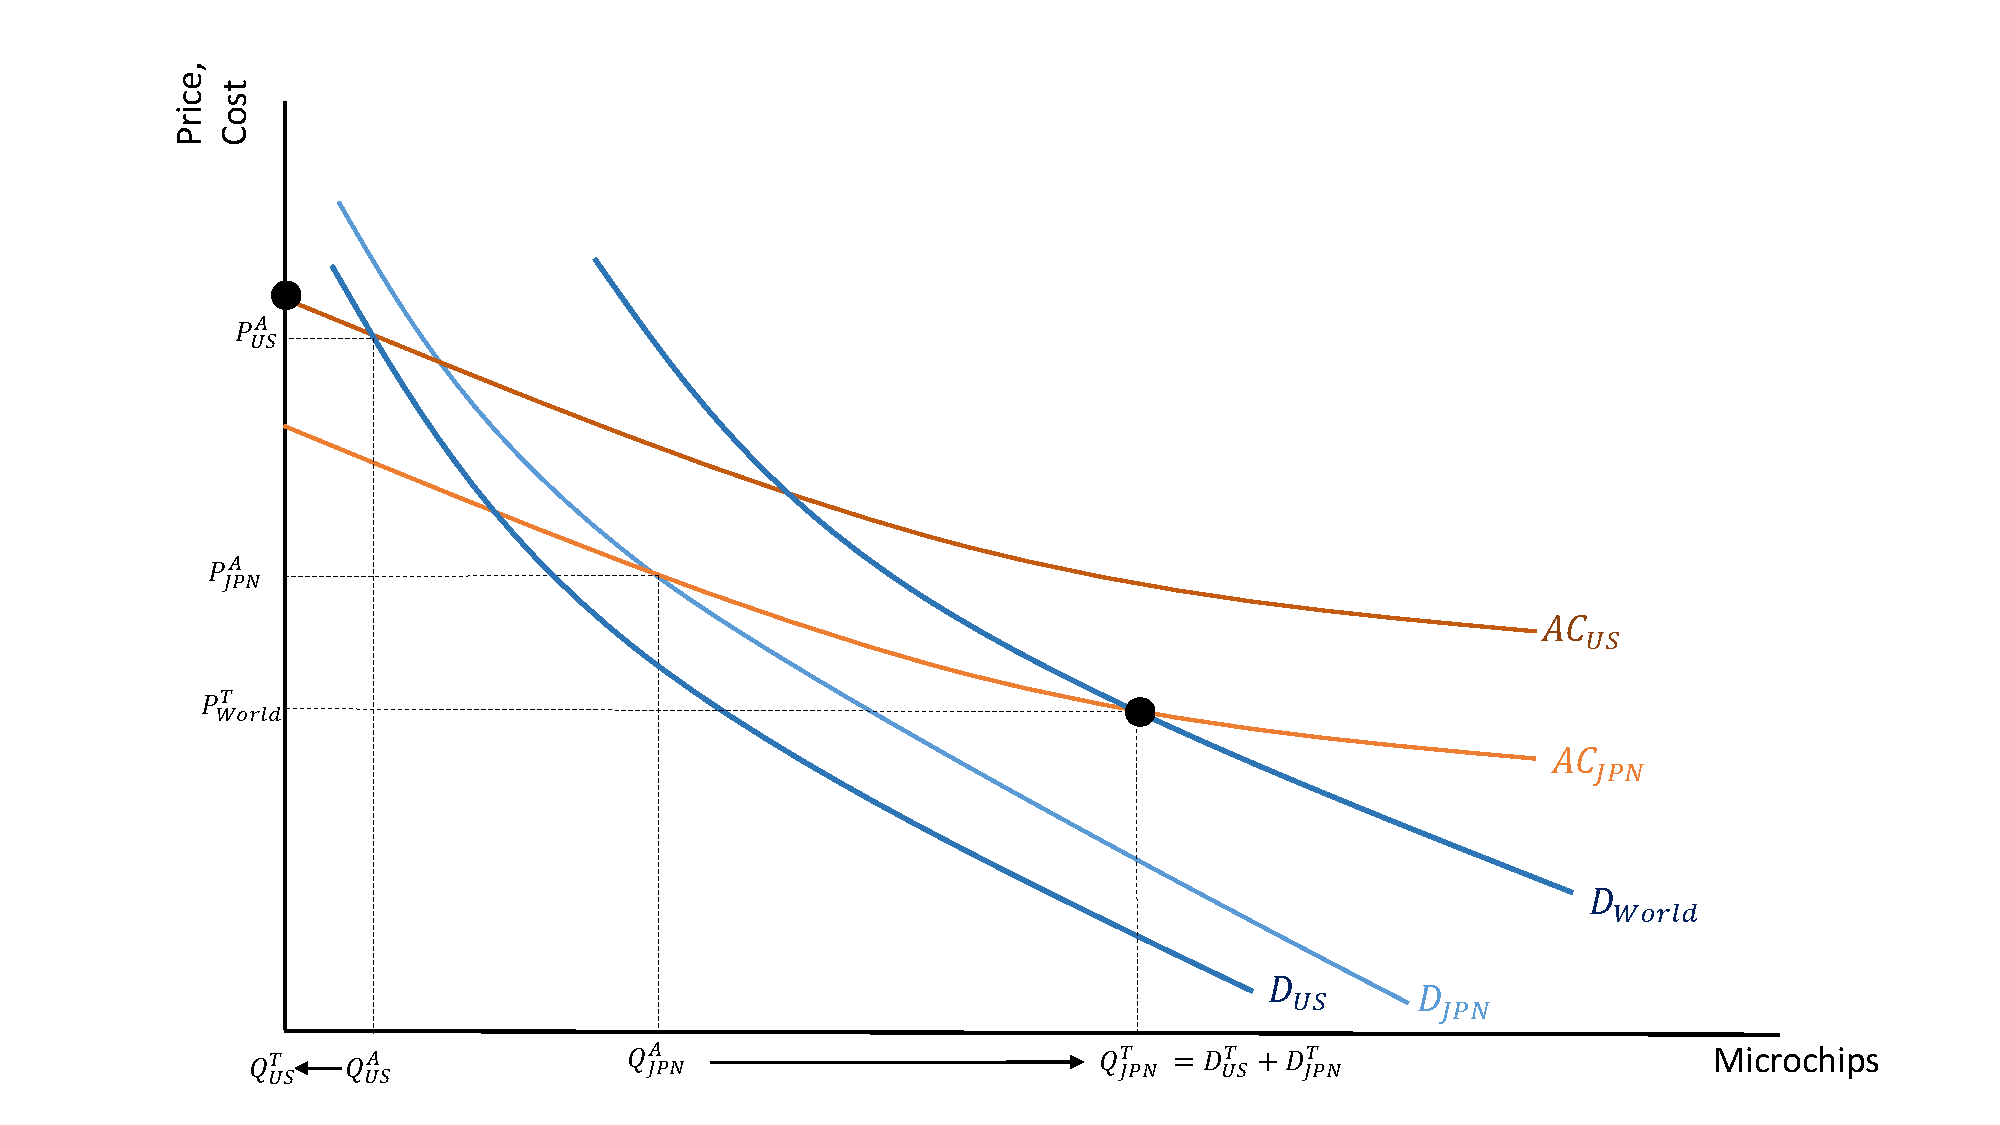
\includegraphics[scale=0.32]{SL4_26.pdf}
\end{frame}

\begin{frame}
	\frametitle{Evaluating the Infant Industry Argument}
\begin{itemize}
	\item The ``infant industry" argument is a valid case for \emph{temporary} trade protection.
		\begin{itemize}
			\item Greater gains both for home and the rest of world to trade liberalization once the industry is ``mature."
		\end{itemize}
			\item Larger issue is identifying when protection is actually appropriate.
				\begin{itemize}
			\item E.g. Trade protection would not help Japan if the U.S. had a much larger market. 
			\item How do we know when an economy has a cost advantage?
				\end{itemize}
\end{itemize}
\end{frame}


\begin{frame}
	\frametitle{Conclusion}
What have covered today:
\begin{itemize}
	\item Increasing returns and firm heterogeneity
		\begin{itemize}
			\item More productive firms with self-select into exporting if it is costly.
			\item Decreased export costs lead to increased competition, creating allocative gains from trade as high-cost firms exit the domestic market.
		\end{itemize}
	\item Empirics
		\begin{itemize}
			\item Both selection and within firm improvements matter for explaining trade induced productivity growth.
		\end{itemize}
	\item External returns to scale. 
		\begin{itemize}
			\item Generates efficiency gains from trade due to increasing returns to scale.
			\item ``Lock-in" made lead to inefficiencies, which trade barriers may help alleviate. 
		\end{itemize}
	
\end{itemize}
\end{frame}















\end{document}